\documentclass[../main]{subfiles}
\ifSubfilesClassLoaded{
    \dominitoc
    \tableofcontentsfile
	\pagenumbering{arabic}
    \setcounter{page}{1}
	\setcounter{chapter}{4}
	\addbibresource{../Biblio/biblio.bib}
}{}


\begin{document}
\chapter{Analyse de l'auto-organisation de CxSOM sur des cartes en une dimension}\label{chap:analyse}
\graphicspath{{06-Analyse/figures},{./figures}}
\minitoc

\`A partir de la méthode expérimentale et de représentation du comportement de l'architecture que nous avons présentée précédemment, nous nous concentrons dans ce chapitre sur l'identification des dynamiques et comportements d'apprentissage d'une architecture CxSOM.
Nous chercherons d'abord à caractériser l'organisation d'architecture de deux et trois cartes en une dimension en étudiant différentes dispositions d'entrées.
Nous introduirons ensuite un comportement spécifique à CxSOM~: la prédiction d'entrée. Nous montrerons que la relaxation permet de prédire une entrée manquante, conférant à des cartes de Kohonen une capacité de prise de décision. Nous appliquerons cette propriété de prédiction de CxSOM au contrôle d'un drone.

\section{Méthode expérimentale}

Nous reprenons dans ce chapitre l'expérience déjà présentée sur le cercle en deux dimensions et étudions quelques autres dispositions géométriques d'entrées.
Ces modèles d'entrées jouet nous permettent de maîtriser les dépendances sur des modalités en basse dimension et ainsi de visualiser les liens entre organisation et apprentissage. 
Cela nous permettra également de mesurer l'apprentissage de cette dépendance connue au sein des structures de cartes.

\subsection{Modèle d'entrées}

Rappelons la définition des entrées multimodales~: il s'agit d'un ensemble d'entrées $\mathbf{\inpx} = (\inpx\m{1}, \cdots, \inpx\m{n})$. Nous notons $K$ la dimension totale des entrées.
Nous représentons la dépendance entre entrées en choisissant une variable latente du modèle $U$ telle que :
$$ \forall i, \inpx\m{i} = f\m{i}(U) + \epsilon\m{i}$$
avec $\epsilon\m{i}$ un bruit sur les entrées.
La dimension de $U$ détermine la dépendance entre les entrées.
Une variable $U$ en une dimension paramètre des points placés sur une courbe~; $U$ en 2 dimensions paramètre une surface. Plus généralement, une variable $U$ de dimension $k$ paramètre des entrées de dimension totale $K > k$, positionnées sur une variété de dimension $k$.

Ce modèle est général~: au pire, la dimension de $U$ correspond à la dimension totale des entrées. 
Par ailleurs, de nombreux modèles d'entrées réelles se placent effectivement sur une variété de dimension réduite. Le choix d'un modèle d'entrées géométriques situées sur une variété de dimension inférieure est donc justifié comme modèle expérimental simplifié.

Une architecture CxSOM est composée de $N$ cartes connectées entre elles, pouvant prendre ou non une entrée externe $\inpx\m{i}$. L'objectif de l'architecture est d'appendre une représentation des relations entre les modalités $\inpx\m{i}$.
Dans cette série d'expériences, nous étudions un modèle d'entrées dans lequel chaque modalité $\inpx\m{i}$ est en une dimension. Chaque carte $M\m{i}$ prend donc une entrée externe $\inpx\m{i}$ en une dimension.

Nous reviendrons d'abord sur le modèle du cercle (\textbf{A}), déjà présenté au chapitre \ref{chap:repr}. L'intérêt de cette courbe est que la disposition est symétrique~: toute entrée $X^{(1)}$ correspond à deux valeurs possibles pour $X^{(2)}$ et inversement. $U$ est une variable 1D.
Nous testerons ensuite si les observations réalisées sur le modèle du cercle se retrouvent pour d'autres dispositions d'entrées, représentées en figure~\ref{fig:input_list}~:
\begin{itemize}
	\item Une entrée est une fonction de l'autre~: $\inpx\m{2} = cos(\inpx\m{1})$~(\textbf{B})
	\item Les entrées sont identiques (cas dégénéré) (\textbf{C})
	\item Entrées sur une courbe de Lissajous (\textbf{D})~: une entrée $\inpx\m{1}$ correspond à 4 à 6 valeurs de $\inpx\m{2}$ et inversement.
	\item Entrées totalement indépendantes, prises aléatoirement dans le carré $[0,1]^2$~(\textbf({E})). $U$ est alors une variable 2D correspondant aux entrées.
	\item Entrées sur un anneau \textbf{(F)}. $U$ est alors une variable 1D avec du bruit dans le modèle d'entrées. Une carte de Kohonen classique a comme propriété d'être résistante au bruit sur les données. Ainsi, une carte 1D se dépliant sur un anneau fin en 2D apprendra d'abord une représentation du cercle sous-jacent. Nous voulons vérifier comment cette propriété se vérifie sur l'apprentissage de données par plusieurs cartes.
\end{itemize}

\begin{figure}[h!]
	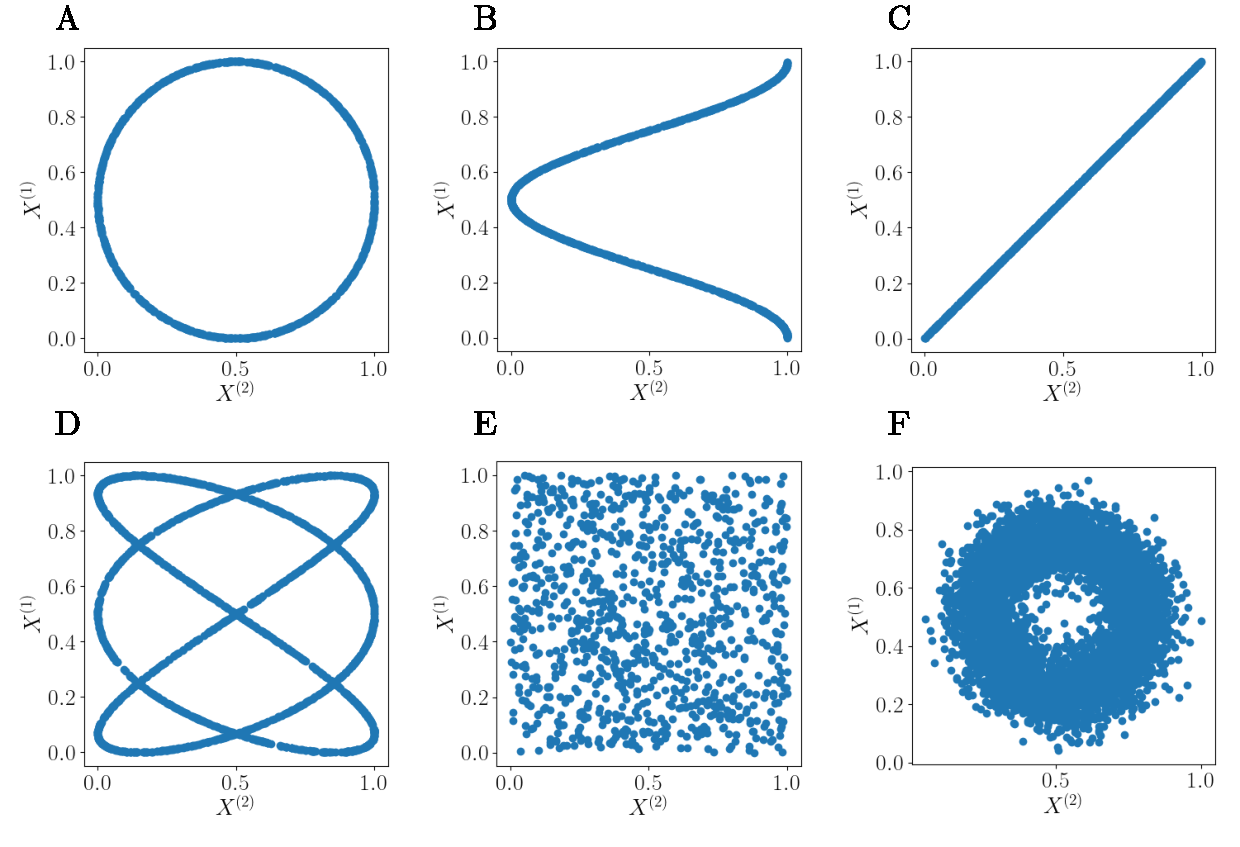
\includegraphics[width=\textwidth]{inputs/inputs.pdf}
	\caption{Dispositions d'entrées en deux dimensions. $M\m{1}$ prend en entrée l'ordonnée $\inpx\m{1}$ et $M\m{2}$ prend en entrée l'abscisse $M\m{2}$. \label{fig:input_list}}
\end{figure}

Nous prendrons ensuite deux configurations d'entrées en trois dimensions, tracées en figure~\ref{fig:inputs_3D} pour les architectures de trois cartes~:
\begin{itemize}
	\item Les entrées sont dans un plan 2D pivoté en trois dimensions. $U$ est une variable 2D.
	\item Les entrées sont sur un cercle en 2D, pivoté en trois dimensions. $U$ est une variable 1D.
\end{itemize}

Dans ces deux cas, la connaissance de deux des entrées ainsi que du modèle détermine la valeur de la troisième entrée. 
Nous étudierons ces configurations dans un cadre de prédiction d'entrées~: nous donnons en entrées $X\m{1}, X\m{2}$ à la structure et regardons si la valeur de $X\m{3}$ correspondante est correctement prédite par l'architecture. 
Une bonne prédiction témoigne de l'apprentissage du modèle d'entrées par l'architecture de cartes.
Les architectures de cartes deux dimensions seront traitées par la suite au chapitre~\ref{chap:analyse2D}.

% \begin{figure}[h!]
% 	\centering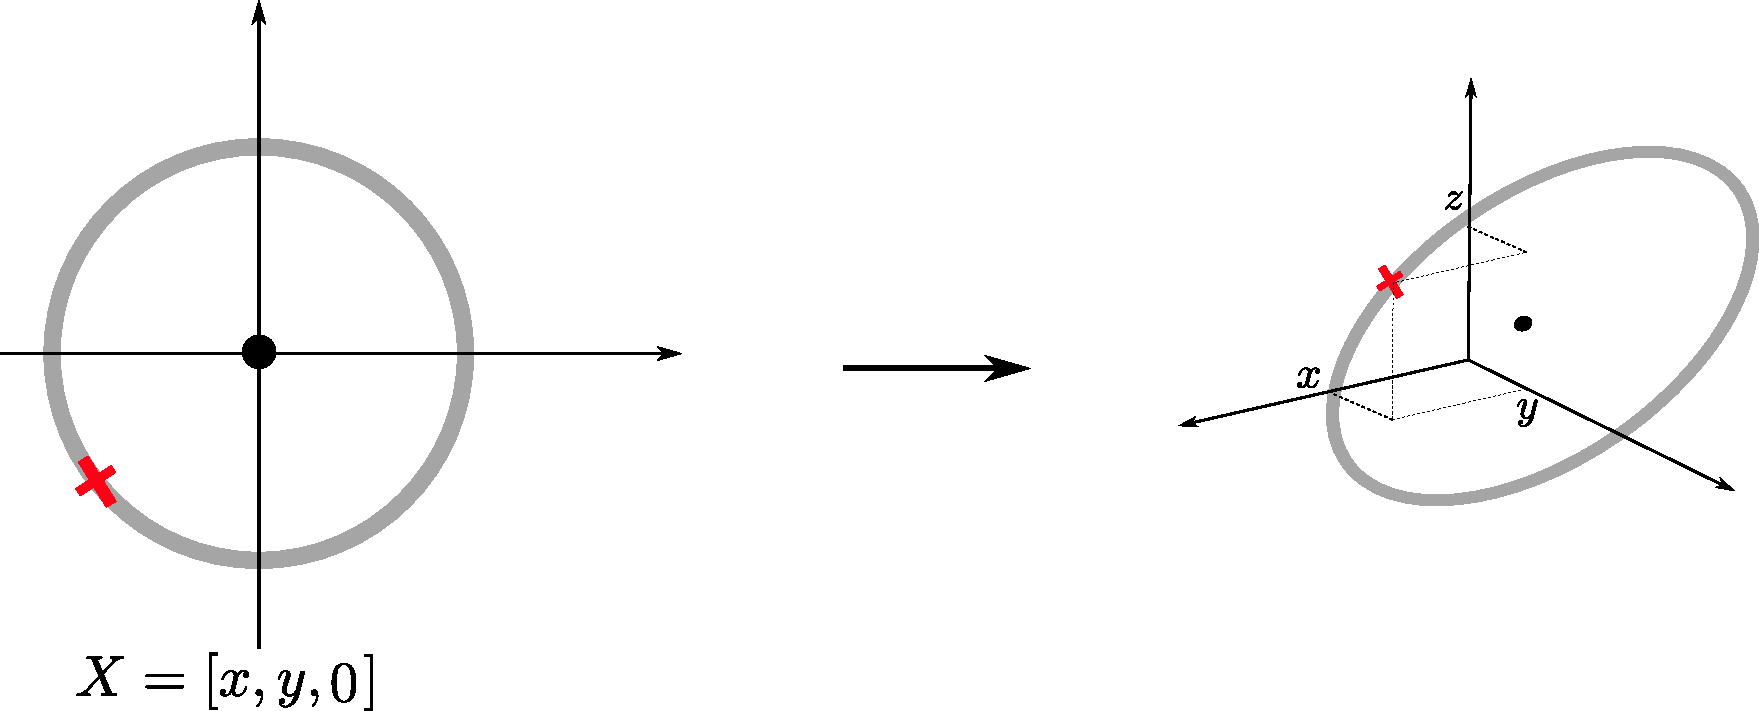
\includegraphics[width=0.9\textwidth]{anneau_inputs.pdf}
% 	\caption{Exemple de courbe plongée en trois dimensions. La figure 2D est pivotée en trois dimensions. Chaque coordonnée est normalisée de façon à s'étendre entre 0 et 1 en trois dimensions.
% 	\label{fig:in_3D}}
% \end{figure}

\begin{figure}[h!]
	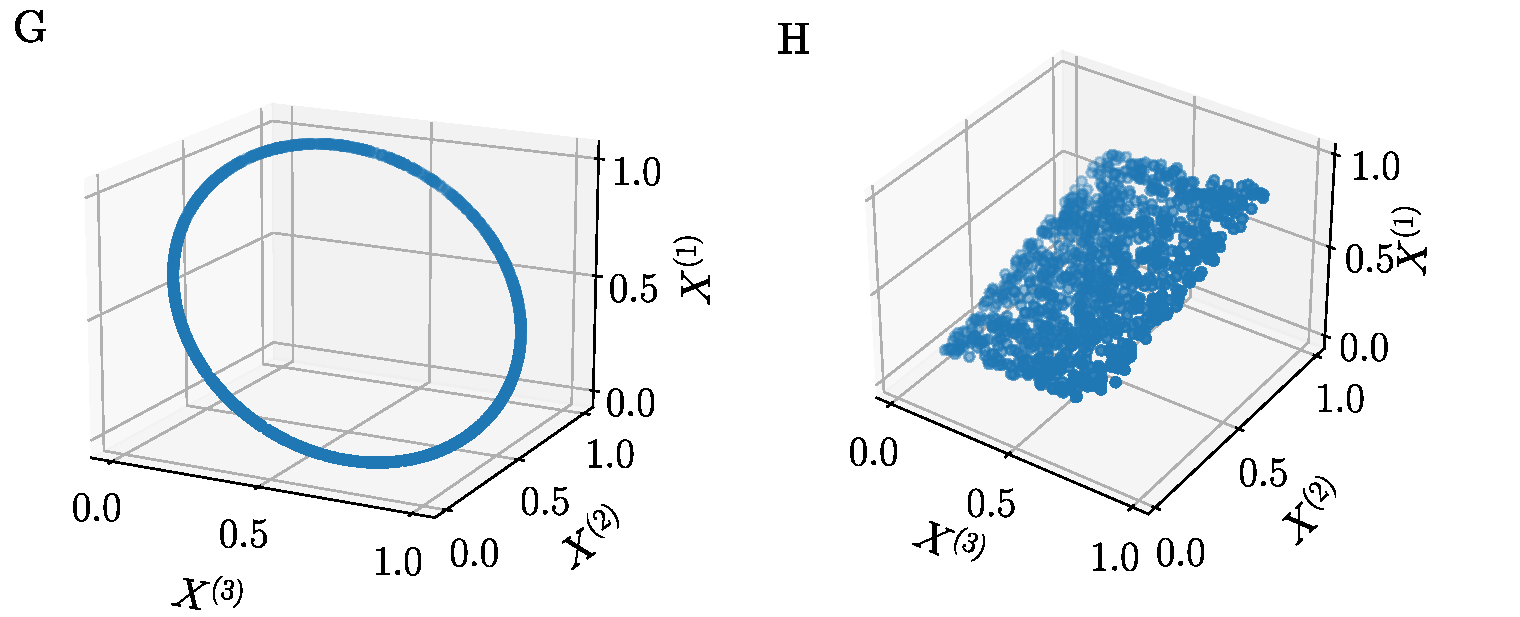
\includegraphics[width=\textwidth]{inputs/inputs_3D.pdf}
	\caption{Dispositions d'entrées en trois dimensions. Chaque carte $M\m{1}$, $M\m{2}$, $M\m{3}$,prend en entrée une coordonnée $\inpx\m{1}, \inpx\m{2}, \inpx\m{3}$. \label{fig:inputs_3D}}
\end{figure}

\subsection{Paramètres des architectures}

Nous étudierons dans ce chapitre des architectures de $N = 2$ et $N=3$ cartes en une dimension. L'étude en 1D facilite les représentations et permet donc une meilleure compréhension des mécanismes d'apprentissage.
Nous considérons des architectures dans lesquelles chaque carte prend une entrée externe. 
Sauf si précisé, les connexions sont réciproques entre chaque carte de l'architecture, ce qui est illustré en figure~\ref{fig:archis}.

\begin{figure}[h!]
	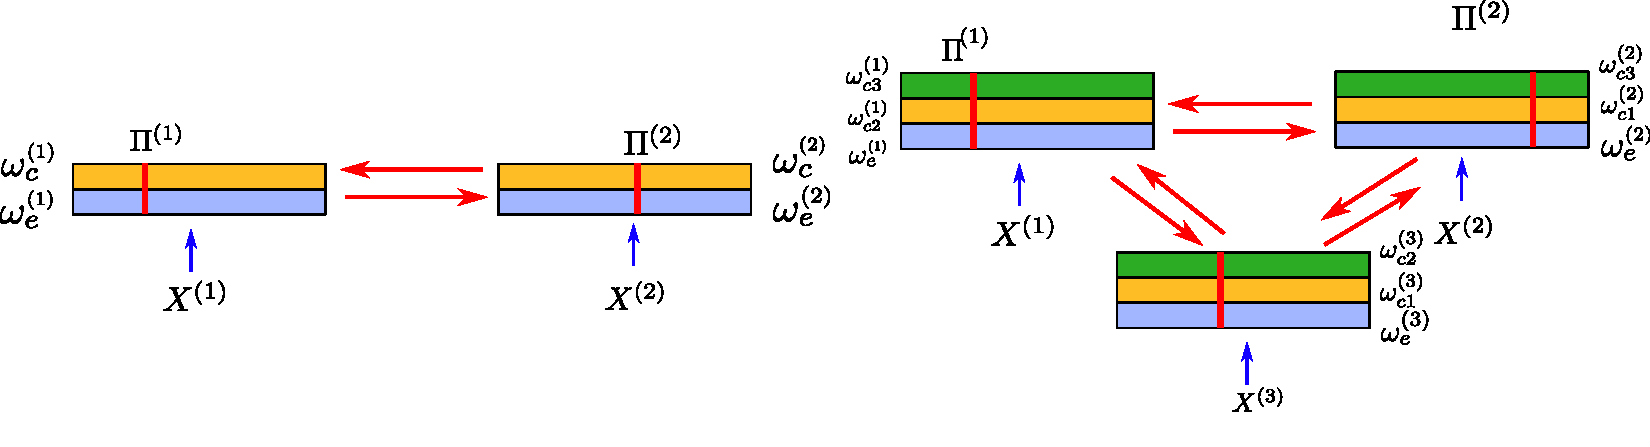
\includegraphics[width=\textwidth]{archis.pdf}
	\caption{Disposition des cartes et connexions des architectures de deux et trois cartes étudiées dans ce chapitre \label{fig:archis}}
\end{figure}

Nous nous concentrons d'abord sur des architectures de deux cartes, prenant chacune en entrée une modalité en une dimension.
Chaque carte a une taille fixée de 500 n\oe{}uds, indexées entre 0 et 1, et possède deux couches de poids $\w_e$ et $\w_c$. Les rayons de voisinage sont fixés à $r_e = 0.2$ et $r_c = 0.02$, sauf si précisé dans l'expérience.

La génération des entrées suit le processus suivant~: $U$ est tiré uniformément dans $[0,1]$, puis les entrées $\inpx\m{1}$ et $\inpx\m{2}$ sont calculées à partir de la valeur de $U$. 
L'apprentissage est réalisé sur un échantillon de 20000 points, générés aléatoirement et présentés une fois. Notons que ce nombre d'exemples est souvent largement supérieur au nombre d'itérations effectivement nécessaires à la convergence des poids. 
Les tests sont ensuite réalisés sur 1000 points générés aléatoirement selon la même distribution d'entrées.

\subsection{Matériel}

Le modèle d'architecture CxSOM est implémenté en C++ en s'appuyant sur la librairie CxSOM \footnote{\url{https://github.com/HerveFrezza-Buet/cxsom}}, développée au sein de notre équipe.
Cette librairie permet d'implémenter des cartes de Kohonen simples ainsi que des architectures CxSOM spécifiquement.
Cette librairie s'interface avec un module python (\emph{pycxsom}) afin de faciliter les représentations et manipulation des cartes pendant et après l'apprentissage.
CxSOM permet de paralléliser au maximum les opérations indépendantes. Par exemple, la phase d'apprentissage des cartes est séquentielle car le calcul des valeurs des poids pour l'itération $i$ dépend de $i-1$, mais toutes les opérations de tests dans lesquelles le temps n'intervient pas tournent en parallèle.
Notons que la gestion du consensus lors de la relaxation passe également par des mécanismes locaux aux cartes dans notre implémentation. 
Nous devons en effet vérifier lors de chaque pas de relaxation si les cartes ont atteint un consensus. Pour cela, chaque carte envoie un signal supplémentaire aux cartes voisines indiquant si son BMU a été modifié. Lorsque qu'une carte reçoit de toutes ses voisines que leur BMU n'est plus modifié et que le BMU de la carte n'a pas non plus été modifié lors de l'étape, la relaxation s'arrête dans cette carte.
Les codes C++ et python que nous avons utilisé pour générer les expériences présentées dans ce chapitre sont disponibles sur git : REF.
Le développement de la librairie CxSOM a été effectué en parallèle de cette thèse. 
Toutes les expériences présentées ici tournent sur un processeur i7 4 c\oe{}urs.



\section{Mécanismes d'auto-organisation jointe sur une architecture de deux cartes}

Le premier but de cette étude est d'identifier des comportements \emph{systémiques} émergeant d'une architecture simple à deux et trois cartes, sur des entrées en deux et trois dimensions. Nous présentons d'abord les comportements relevés sur le modèle d'entrées \textbf{A}, puis nous étendrons ces observations aux autres modèles d'entrées.

\subsection{Mécanismes observés sur les entrées en cercle}

Revenons d'abord sur l'expérience précédemment présentée au chapitre \ref{chap:repr}, réalisée sur les entrées disposées selon un cercle (\textbf{A}).
Après avoir vérifié que les poids des cartes convergent au cours de l'apprentissage, nous relèverons les comportements d'apprentissage spécifiques au modèle CxSOM.

\subsubsection{Convergence des poids}

Dans une carte de Kohonen classique, le rayon de voisinage et le taux d'apprentissage sont diminués de façon prédéfinie au cours des itérations. 
Cette opération permet d'assurer un dépliement des cartes au début de l'apprentissage puis assure la convergence des poids $\w$ des cartes lorsque les paramètres sont faibles.
Dans notre étude, nous choisissons au contraire de ne pas modifier les paramètres d'apprentissage au cours des itérations.
Nous vérifions dans cette section la convergence des poids des cartes avant d'étudier l'organisation. 

La figure~\ref{fig:conv} présente l'évolution des variations des poids $\w\ext$ et $\w\cont$ dans chaque carte au cours de l'apprentissage. Toutes les 100 itérations, nous calculons la différence maximale entre $w_t$ et $w_{t-100}$.
Nous observons que cette courbe tend vers $0$ pour chaque courbe de poids. Cela montre que tous les poids de la carte tendent vers une position stable.

Les observations montre qu'une carte se comporte d'abord comme une carte de Kohonen classique apprenant sur des entrées externes, ce qui s'explique par la différence de contribution dans l'activité globale des activations externes et contextuelles, calculée par~: 
$$ a_g = \sqrt{a_e \cdot (\beta a_e + (1-\beta)a_c)}$$
Les entrées contextuelles viennent seulement moduler le calcul de l'activité externe.
Notons toutefois que nous sommes sur un cas particulier de cartes 1D sur des entrées 1D.
La convergence en l'absence de décroissance de paramètres peut poser plus de problèmes sur des cartes en deux dimensions. 
Nous verrons que pour des rayons de voisinage bien choisis, la convergence sera possible également en deux dimensions.

\begin{figure}[h!]
	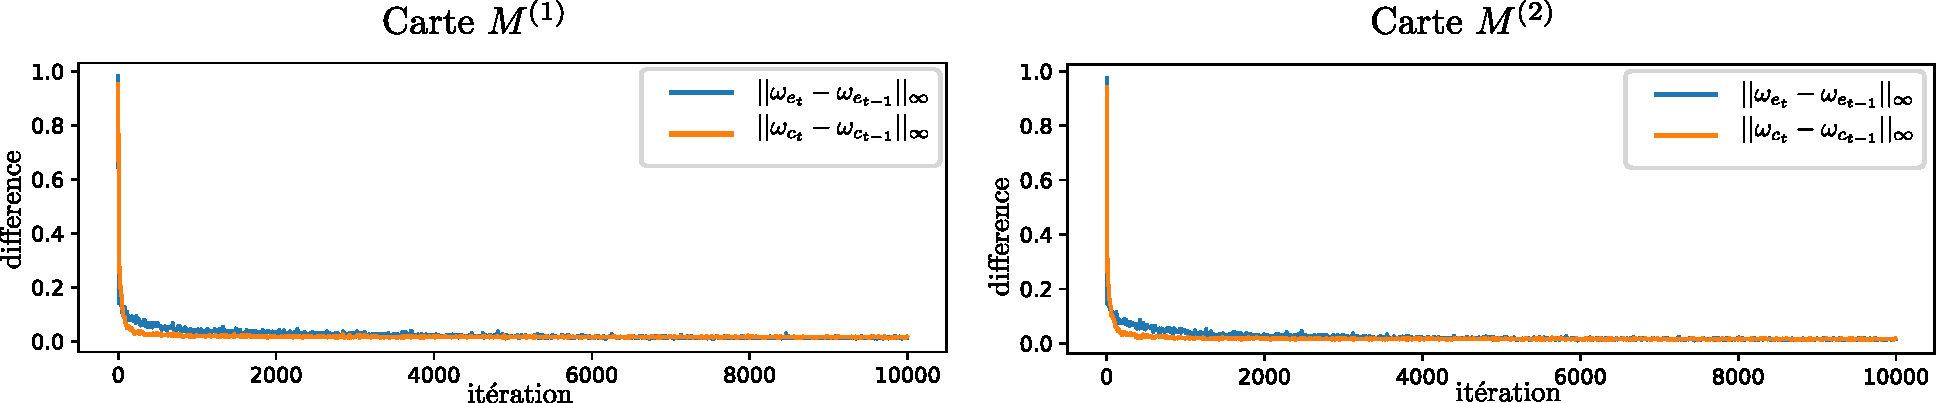
\includegraphics[width=\textwidth]{convergence/cercle_moy.pdf}
	\caption{Pour chaque carte, nous représentons l'évolution en fonction du temps d'apprentissage, de la différence maximale en valeur absolue entre les poids à l'instant $t$ et ceux à $t-100$ $\w_t$ et $\w_{t-100}$. Les entrées sont ici un cercle en deux dimensions. L'évolution est moyennée sur 10 apprentissages dont les entrées sont tirées aléatoirement selon la même distribution, un cercle en deux dimensions.
	Ces tracés montrent que les poids externes et contextuels convergent rapidement vers une position stable.\label{fig:conv}}
\end{figure}


\subsubsection{Disposition des poids}

Nous nous intéressons à présent à l'organisation des cartes lorsque les poids ont convergé.
Les poids, les entrées et les BMUs associés sont tracés en figure~\ref{fig:w} selon la représentation cartographique décrite au chapitre \ref{chap:repr}.
Les poids externes, en orange, présentent une disposition similaire à ceux observés dans une carte classique : ils sont classés de façon monotone entre 0 et 1.
Les poids contextuels, en bleu, présentent une forme de \og vagues \fg{}. 

Les entrées sont tracées en fonction des positions de BMUs associées en rose et vert. 
Nous observons que les positions des BMUs dans la carte $M\m{1}$ se répartissent en zones, séparées par des zones mortes dont les n\oe{}uds n'ont jamais été BMUs.
C'est une première différence avec une carte classique, pour laquelle toutes les positions seront BMUs lorsque les entrées sont distribuées de façon continue.
Les zones dans lesquelles les n\oe{}uds sont BMUs correspondent aux extrema des poids contextuels et leurs alentours.

\begin{figure}[h!]
	\centering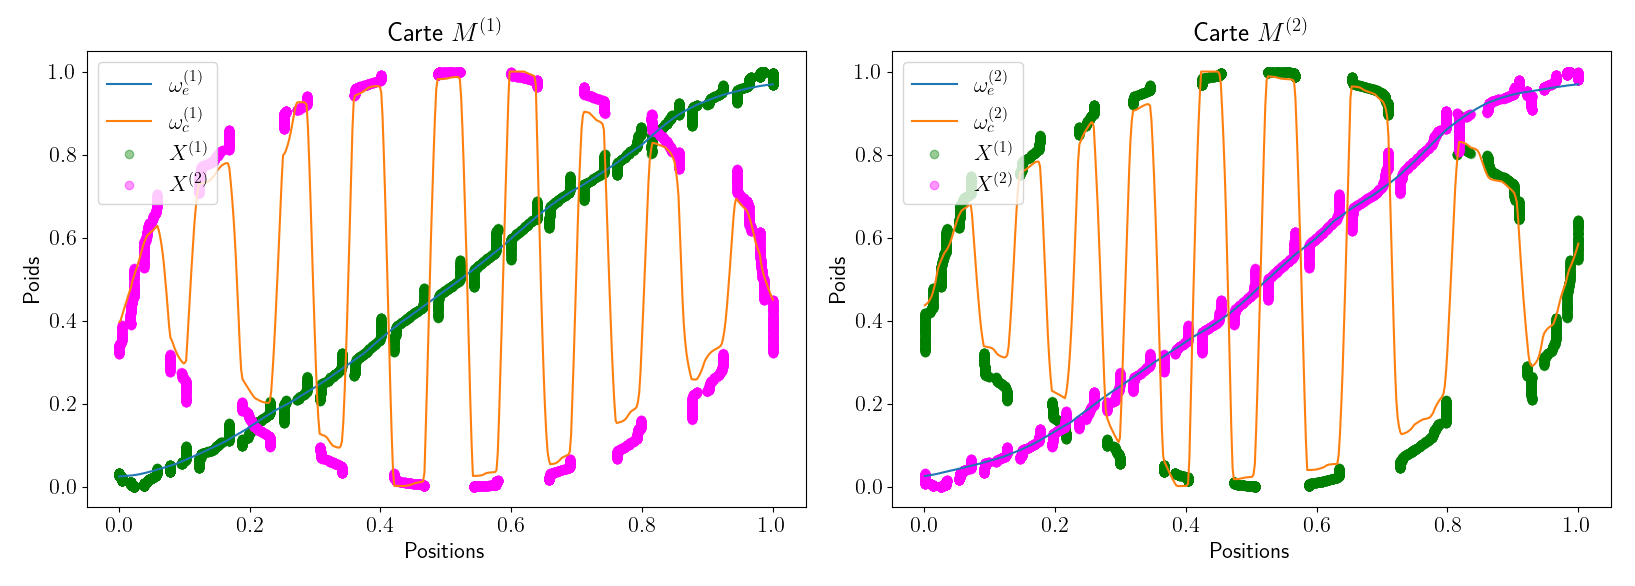
\includegraphics[width=\textwidth]{cercle/weights_1000.png}
	\caption{Représentation cartographique des poids et entrées lors d'une phase de test selon la position dans chacune des cartes. Nous remarquons que les poids d'une carte, par exemple la carte $M^{(1)}$ s'organisent en zones différenciant les valeurs de la paire $X^{(1)}, X^{(2)}$ et non seulement de la valeur de $X^{(1)}$. Deux zones adjacentes codent pour des valeurs de $X^{(1)}$ proches, mais $X^{(2)}$ différents. Au sein d'une même zone, les BMUs s'organisent sous la forme d'une sous-carte auto-organisée sur les valeurs de l'entrée contextuelle. Ces zones se forment de manière auto-organisée. \label{fig:w}}
\end{figure}


La figure~\ref{fig:w_zoom} est un grossissement de quatre zones de la carte $M\m{1}$.
Cette figure montre que les zones définies par les poids contextuels partagent les positions des BMUs en fonction de la valeur des entrées. 
Les deux points mis en valeur en rouge et bleu ont la même valeur de $\inpx\m{1}$ mais une valeur différente de $\inpx\m{2}$. Ils ont ici un BMU différent dans la carte $M\m{1}$. Ces BMUs sont situés dans deux zones adjacentes.
Deux zones adjacentes correspondent par ailleurs à des segments de valeur d'entrée externes qui se recouvrent.
Ce phénomène est également observé dans la carte $M\m{2}$.

\begin{figure}[h!]
	\centering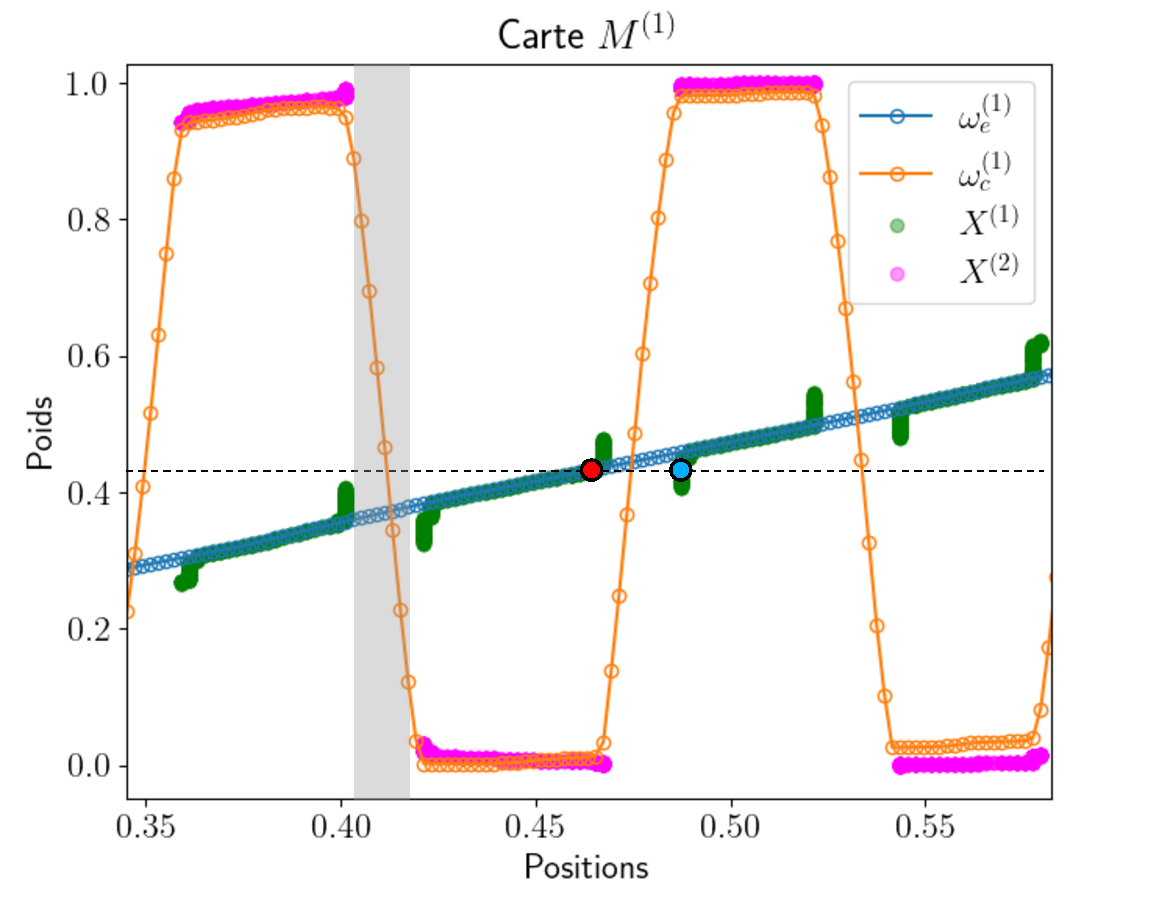
\includegraphics[width=0.45\textwidth]{cercle/weights_zoom_1000_002.pdf}
   \caption{Zoom sur la figure \ref{fig:w} entre les positions 0.35 et 0.55 de la carte $M\m{1}$. 
   Nous y faisons apparaître la position sur la courbe des n\oe{}uds de la carte.
   Deux zones consécutives seront BMUs pour des ensembles d'entrées qui se recouvrent. Par exemple, les deux entrées correspondant au points bleu et rouges ont les mêmes valeurs de $\inpx\m{1}$, mais des valeurs différentes de $\inpx\m{2}$. Leurs BMUs sont alors séparés dans la carte $M\m{1}$ dans deux zones consécutives.
   Entre les zones, quelques unités ne sont jamais BMU, en gris sur la figure. Il s'agit de zones mortes, créant des discontinuités dans la réponse de la carte.
   \label{fig:w_zoom}}
\end{figure}


Dans chaque carte, une position se spécialise donc en tant que BMU par rapport aux entrées externes et à l'entrée contextuelle. C'est bien ce à quoi on s'attend en ayant deux couches de poids. 
Cette différenciation est réalisée par une organisation de la carte en un nombre fini de zones distinctes. Dans chaque zone, les unités sont BMUs pour un segment de valeurs d'entrée externe et contextuelles. Au sein d'une zone, la répartition des entrées externe selon le BMUs est ordonnée, comme ce serait le cas dans une carte auto-organisatrice classique. Le comportement de la carte au sein d'une zone reste donc similaire à celui d'une carte classique.
Il s'agit d'une deuxième échelle d'organisation, qui garde également l'aspect ordonné d'une carte classique. 

Ces zones sont créées par auto-organisation~; aucun paramètre de la carte n'a été modifié pendant l'apprentissage pour former ces zones.

\subsubsection{Erreur de quantification vectorielle}

Nous nous intéressons enfin à la quantification vectorielle réalisée sur l'entrée externe dans chaque carte. Nous souhaitons que le poids externe du BMU soit une approximation de l'entrée externe. Cette quantification permet d'interpréter la sortie d'une carte dans l'espace des entrées, par exemple pour prédire une valeur.

La Figure~\ref{fig:qv} présente la valeur de cette approximation au sein de chaque carte, $\w\ext(\bmu\m{i})$, en fonction de l'entrée correspondante $\inpx\m{i}$. 
Cette figure montre que la quantification vectorielle est bien réalisée~: les valeurs approximées sont proches des valeurs d'entrées.
L'erreur de quantification est plus forte que celle qu'on obtiendrait avec une carte de même taille et mêmes paramètres apprenant sur l'ensemble de $\inpx\m{i}$~. 
Nous remarquons enfin une disposition en étages, dues aux zones formées par les poids contextuels.
Les n\oe{}uds de zones adjacentes de la carte sont en effet BMU pour des intervalles d'entrée qui se recoupent.
Une même valeur d'entrée peut avoir un BMU dans deux zones consécutives de la carte en fonction de la valeur de l'entrée contextuelle. Comme les poids externes sont strictement croissants (ou décroissants), cela induit l'erreur observée dans la prédiction d'entrée.

\begin{figure}[h!]
	\centering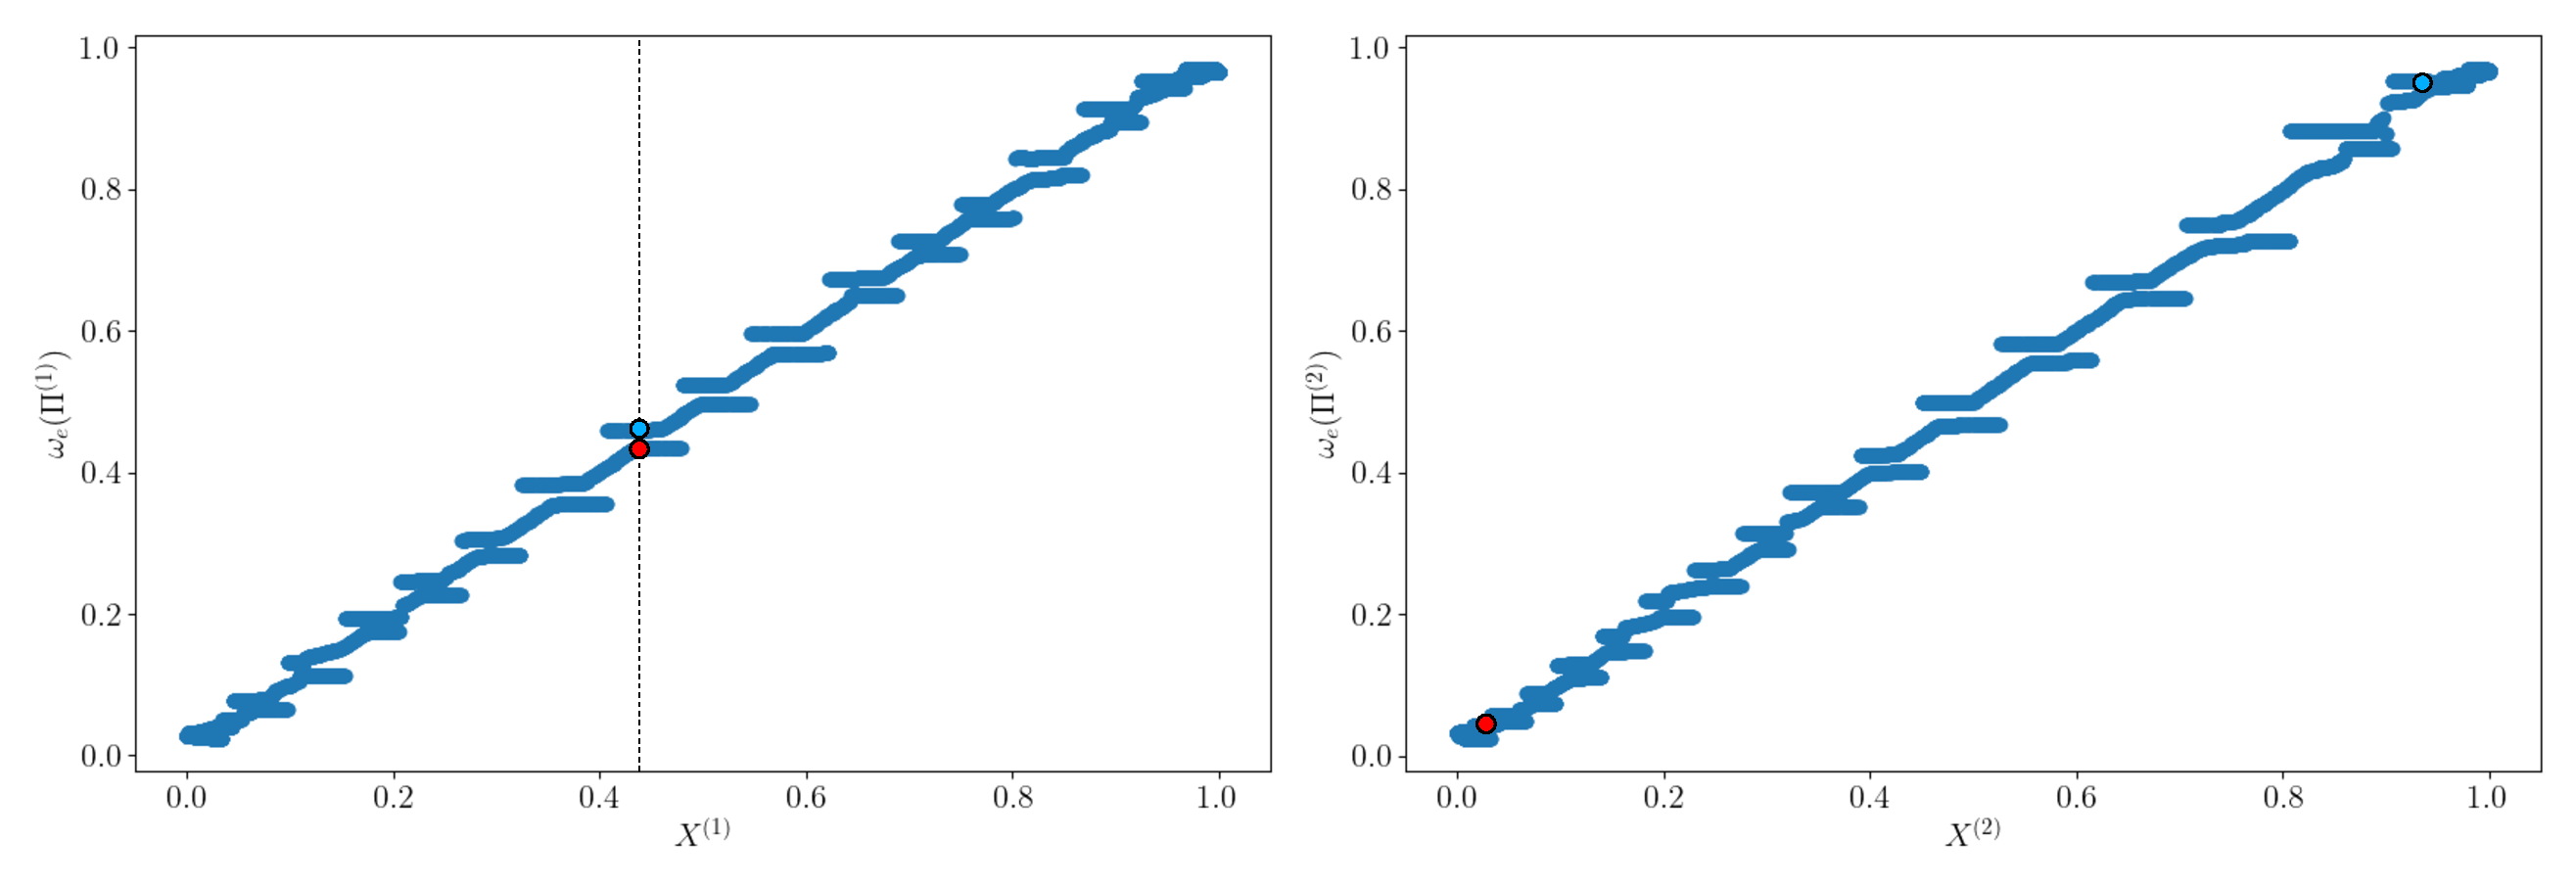
\includegraphics[width=\textwidth]{cercle/frz-error_1000.pdf}
	\caption{Représentation de l'erreur de quantification sur les valeurs de $X^{(1)}$ et $X^{(2)}$. Le poids externe du BMU est proche de la valeur de l'entrée~; chaque carte réalise ainsi une bonne quantification vectorielle sur ses entrées. 
	Les poids rouges et bleus représentés en figure \ref{fig:w_zoom} sont reportés sur le graphique. \label{fig:qv}}
\end{figure}

\subsubsection{Apprentissage du modèle dans chaque carte}

Enfin, au \ref{chap:repr}, nous avons observé que l'apprentissage des relations entre entrées se traduit par une relation fonctionnelle entre $U$ et $\bmu$ dans chaque carte, voir figure \ref{fig:U_BMU}.
Cette propriété traduit l'observation que nous avons faite qu'un BMU se spécialise en fonction de l'entrée externe et des entrées contextuelles.

\subsubsection{Conclusion}

Les résultats de cette expérience ainsi que les observations présentées au chapitre~\ref{chap:representation} nous permettent donc de formuler les hypothèses suivantes concernant le comportement d'architecture de deux cartes en une dimension~:

\begin{itemize}
	\item Chaque carte de l'architecture présente une faible erreur de quantification vectorielle sur ses entrées externes \ref{fig:qv}
	\item Les poids contextuels de chaque carte s'organisent en zones distinctes. Une zone correspond à un même intervalle de valeur pour $\inpx$ et $U$. Deux zones adjacentes encodent le même intervalle de valeurs de $\inpx$ mais des valeurs distinctes de $U$. Ces zones se caractérisent par un étirement de la carte entre deux valeurs éloignées, apportant un aspect discontinu. Cette discontinuité passe en fait par la présence d'une zone peu dense de la carte contenant des n\oe{}uds qui ne seront jamais BMUs. Nous verrons en section \ref{sec:pred} que la formation de ces zones ainsi que la propriété de quantification vectorielle de l'entrée externe permet à la carte de prédire des entrées manquantes.
	\item L'apprentissage du modèle d'entrée par l'architecture se traduit par l'existence d'une relation fonctionnelle entre $U$ et $\bmu$ dans chaque carte, montrant que chaque carte encode l'état de toute l'architecture et non seulement l'état des entrées externes.
\end{itemize}

Nous chercherons à vérifier ces hypothèses sur d'autres dispositions d'entrées dans des structures de deux cartes et de compléter ces observations.
Nous étudierons si les zones dépendent du modèle d'entrées, comment ces zones se forment, et quelles propriétés d'apprentissage elles confèrent à l'architecture de cartes.
Nous introduirons ensuite un comportement possible grâce à l'architecture de cartes~: la prédiction d'entrée manquante.

\subsection{Organisation des cartes en fonction de la distribution d'entrées}

Nous comparons l'organisation des poids et des BMUs sur les différentes dispositions d'entrées.
Dans toutes ces dispositions, nous avons vérifié que la quantification vectorielle est bien réalisée dans chaque carte sur ses entrées. Nous nous concentrerons sur la présence ou non de zones de poids contextuels dans l'organisation finale des poids en fonction de la distribution des entrées.

\subsubsection{Formation de zones selon le modèle d'entrées}

La figure \ref{fig:id_results} présente la disposition des poids et entrées des cartes lorsque $\inpx\m{1}$ et $\inpx\m{2}$ sont identiques (Entrées \textbf{C}).
Dans ce cas, les poids externes et contextuels ne forment pas de zones et les deux cartes se comportent comme une seule carte simple sur $\inpx\m{1} = \inpx\m{2}$. 
En figure~\ref{fig:cos_results}, la dépendance entre les entrées présentée n'est bijective~: $\inpx\m{2}$ est fonction de $\inpx\m{1}$, mais pas l'inverse (Entrées \textbf{B}). 
La carte $M\m{1}$ ne forme pas de zones, car une seule valeur de $\inpx\m{2}$ correspond à une même valeur de $\inpx\m{1}$.
Au contraire, la carte $M\m{2}$ doit à présent se diviser pour apprendre les deux valeurs de $\bmu\m{1}$ possibles correspondant à $\inpx\m{2}$. 
Ce comportement rejoint ainsi celui observé sur le cercle.

\begin{figure}[h!]
	\centering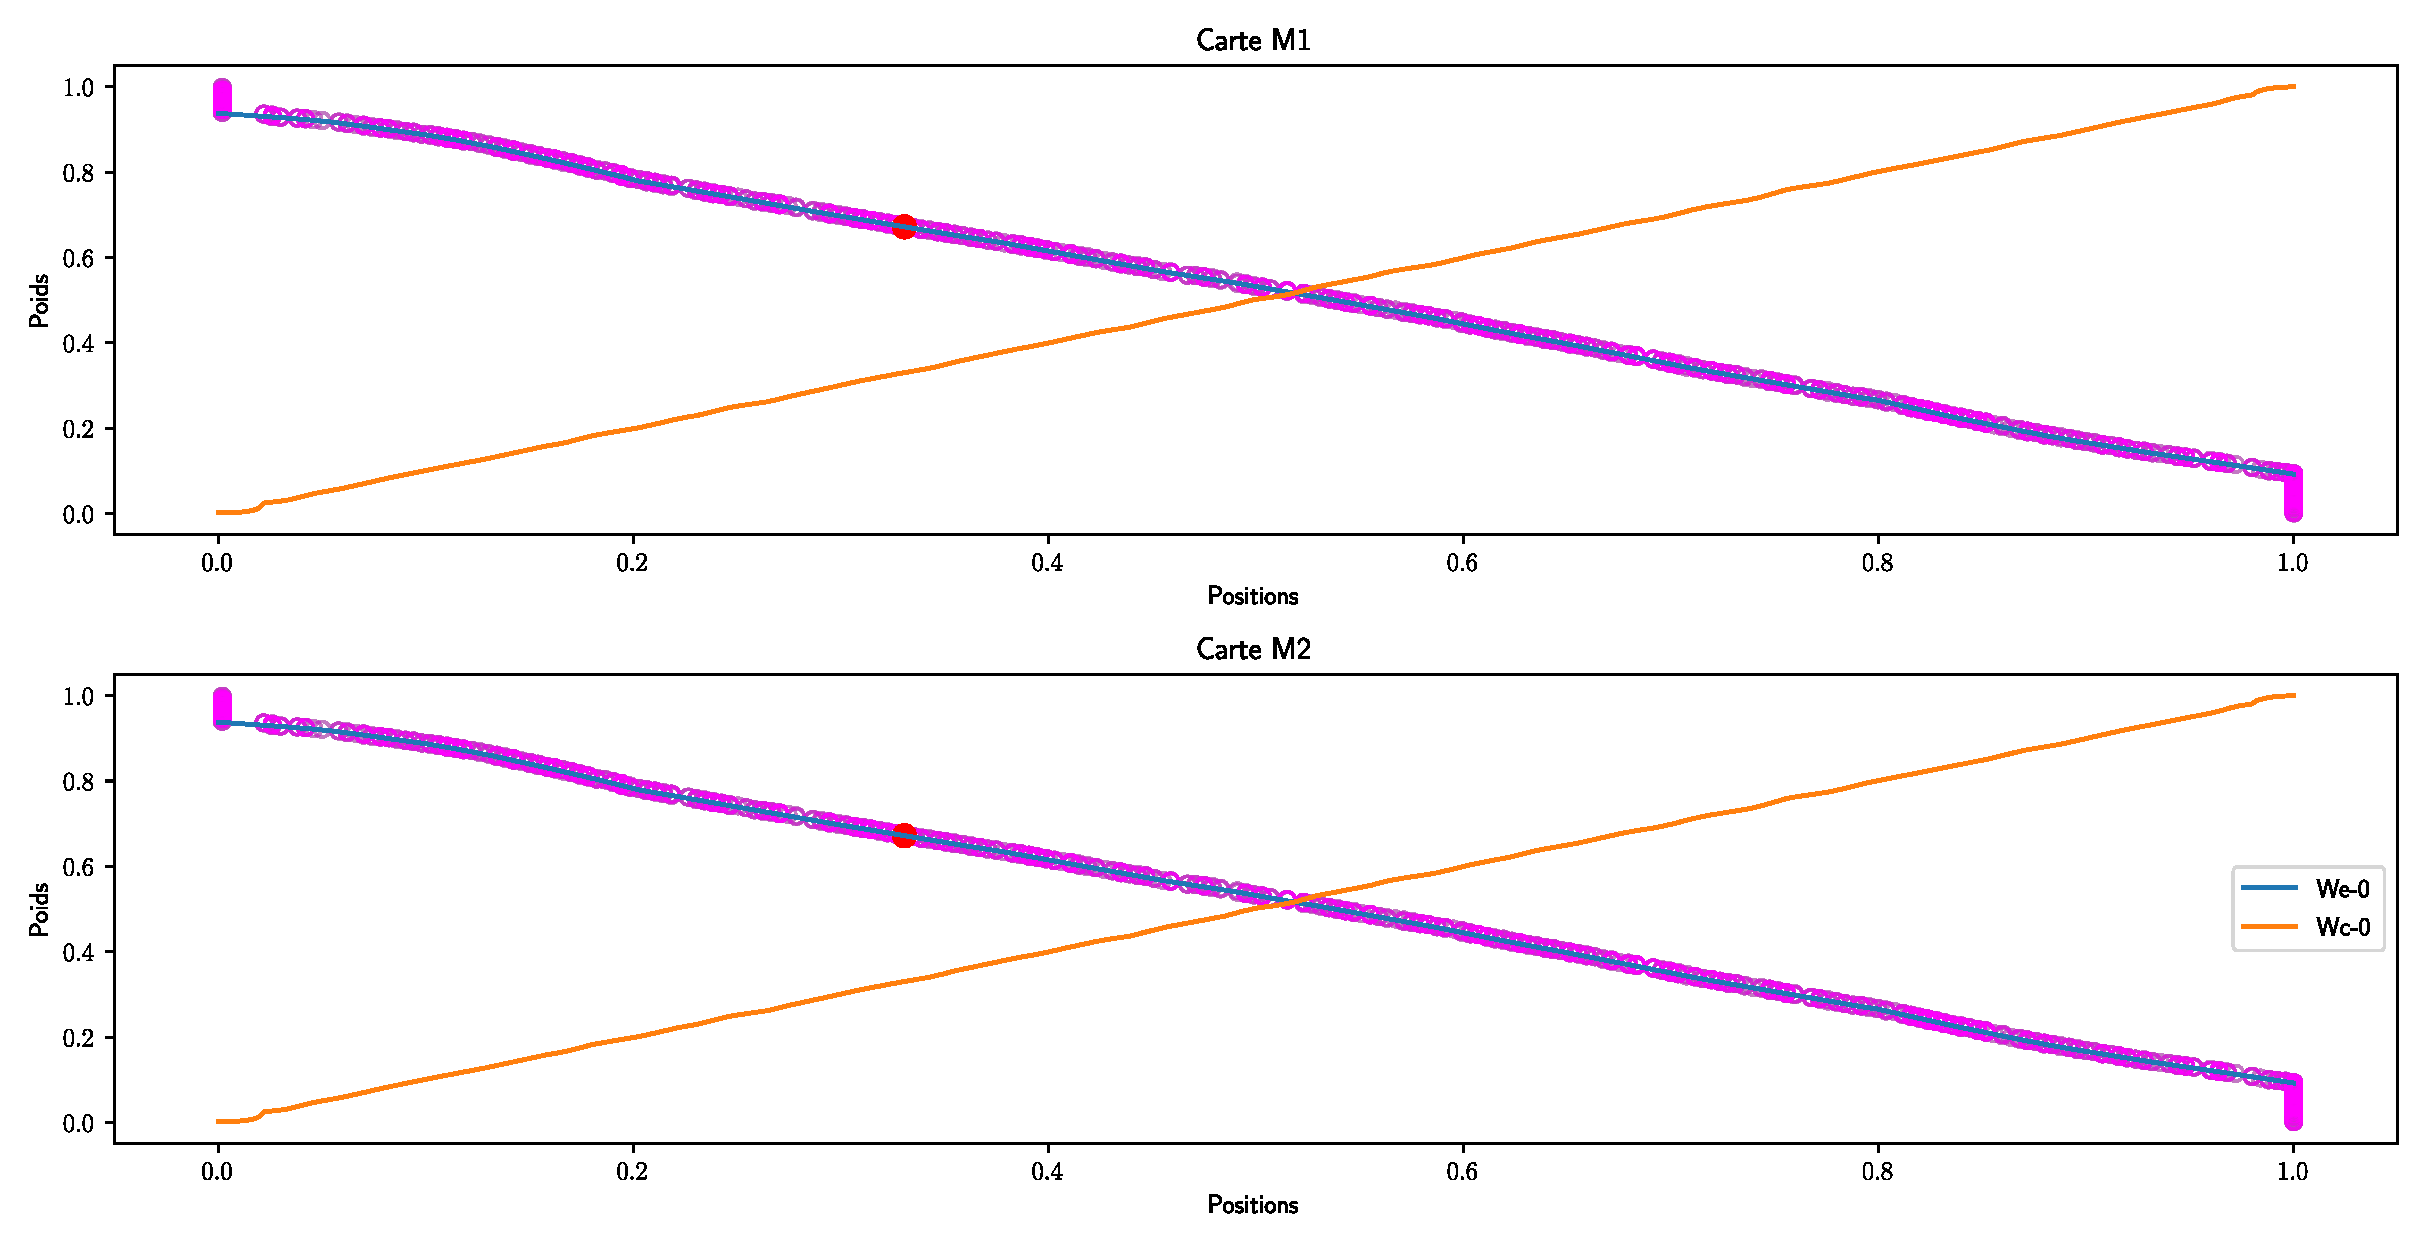
\includegraphics[width=\textwidth]{2som_id_w.pdf}
	\caption{Représentation cartographique des poids et entrées pour la disposition identité. Les poids externes et contextuels sont superposés, et les poids contextuels n'ont pas besoin de former de zones \label{fig:id_results}}
	\end{figure}
	
	\begin{figure}[h!]
		\centering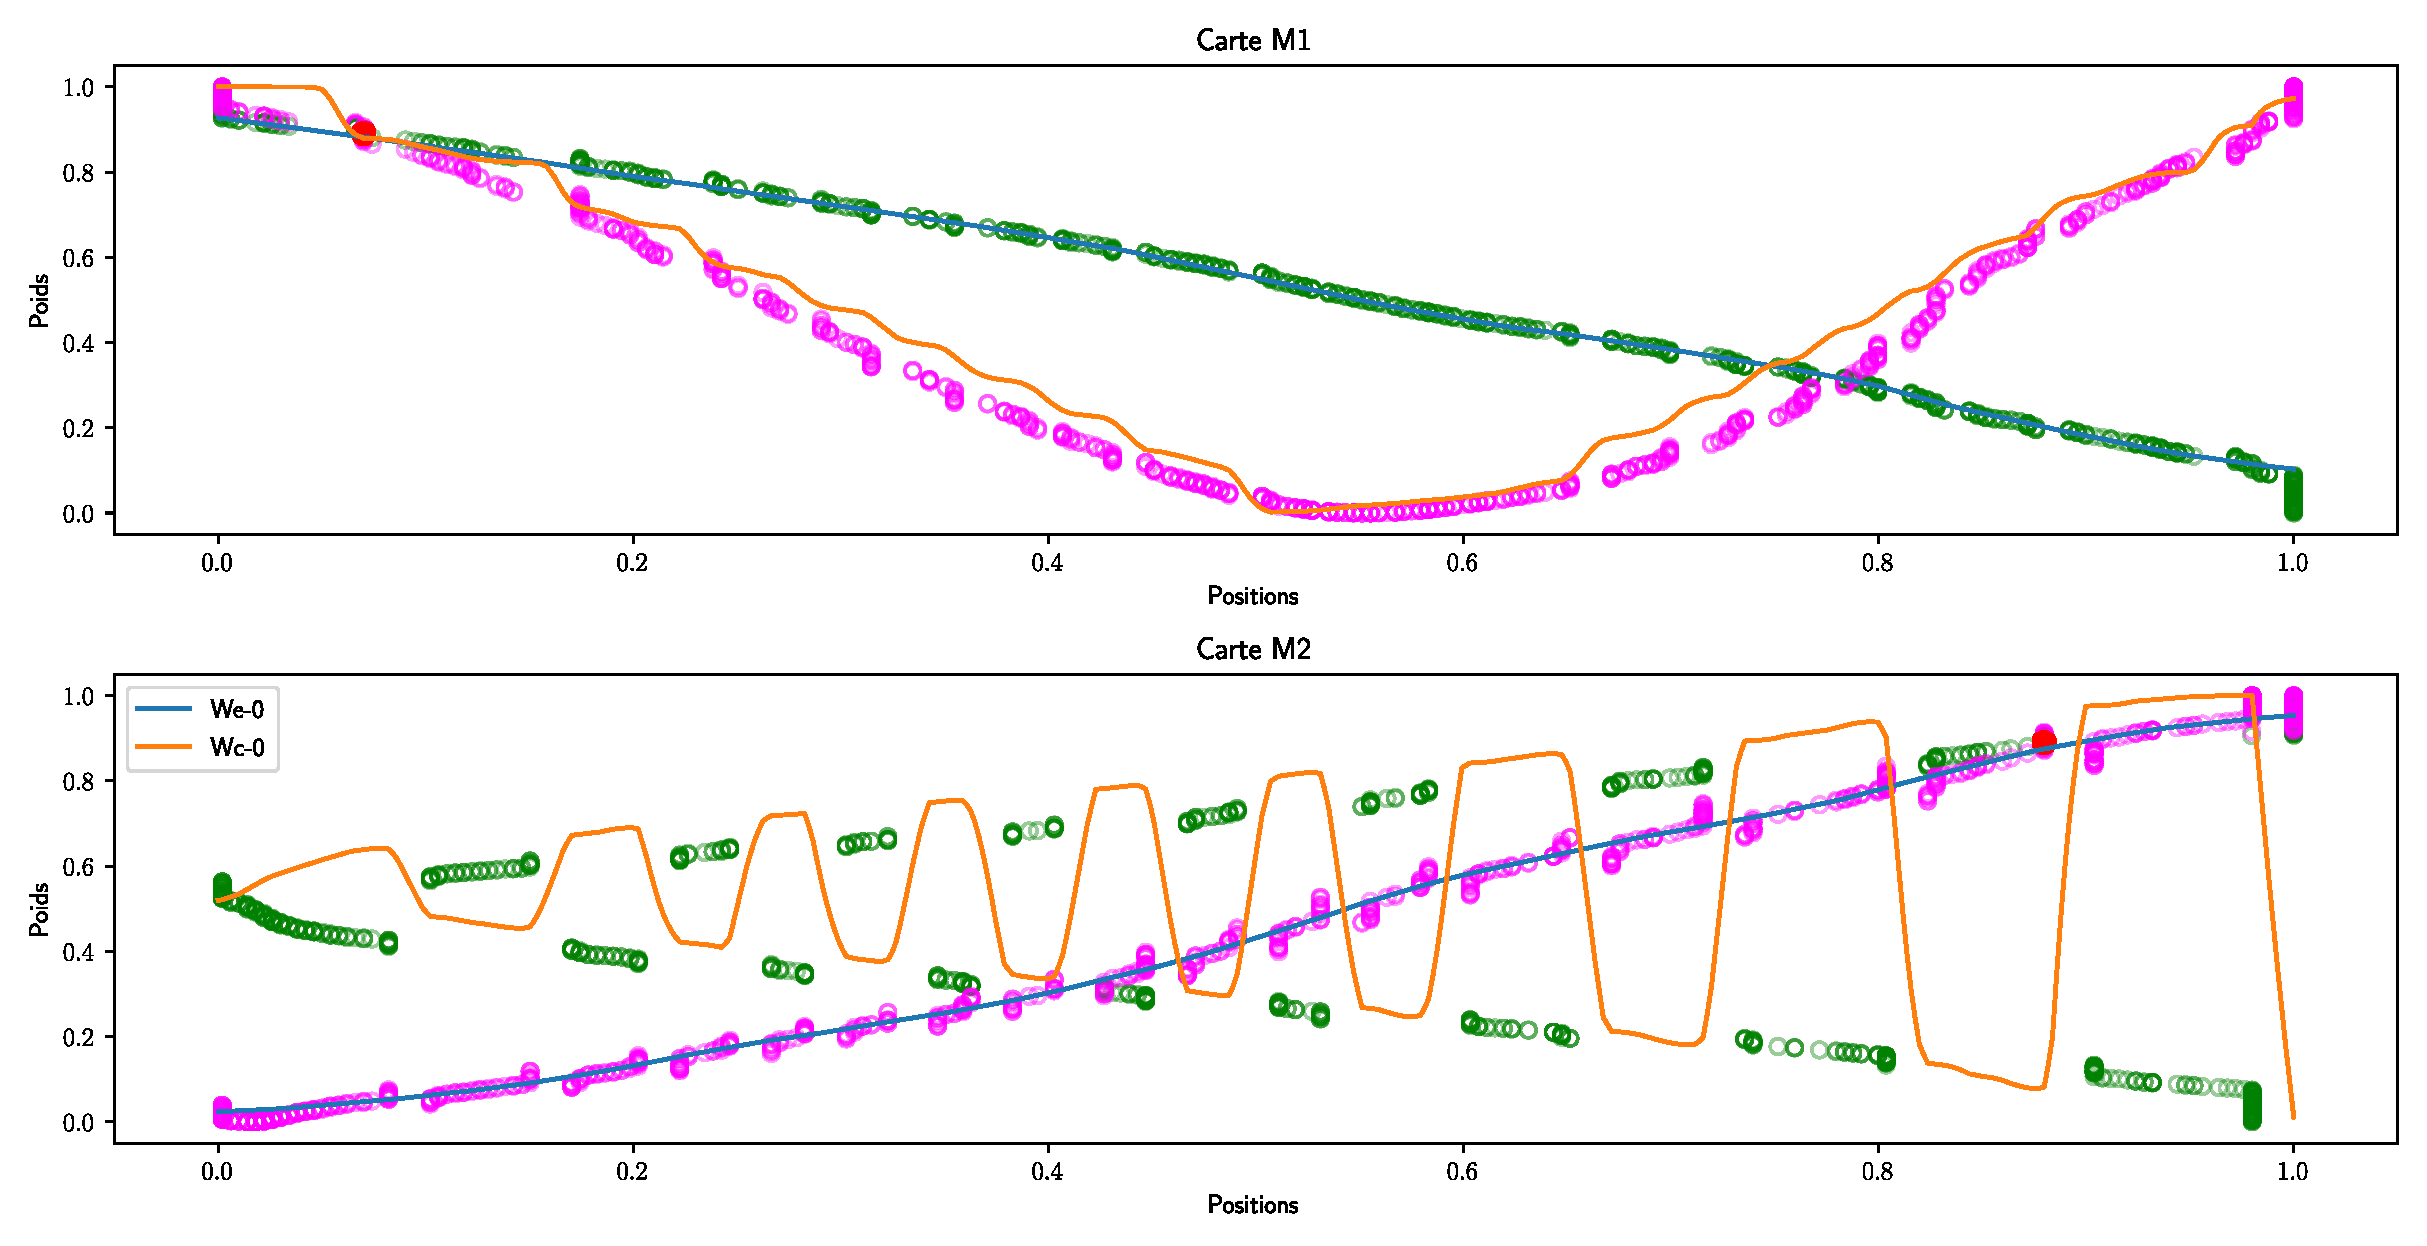
\includegraphics[width=\textwidth]{2som_cos_w.pdf}
		\caption{Représentation cartographique des poids et entrées pour $\inpx\m{2} = cos(\inpx\m{1}$. Les poids contextuels de la carte $M\m{1}$ ne forment pas de zones car une seule valeur de $\inpx\m{2}$ correspond à une entrée $\inpx\m{1}$. Au contraire, les poids de la carte $M\m{2}$ s'organisent pour gérer la distinction. \label{fig:cos_results}}
	\end{figure}

Regardons maintenant l'organisation des cartes lorsqu'une valeur de $\inpx\m{1}$ correspond à plus de valeurs de $\inpx\m{2}$~: 4 dans le cas de la courbe de Lissajous (Entrées \textbf{B}) ou tout l'intervalle $[0,1]$ dans le cas du patch $[0,1]^2$ (Entrées \textbf{E}). Ces organisations sont tracées en figure~\ref{fig:lissa} et \ref{fig:ind}.

\begin{figure}[h!]
	\centering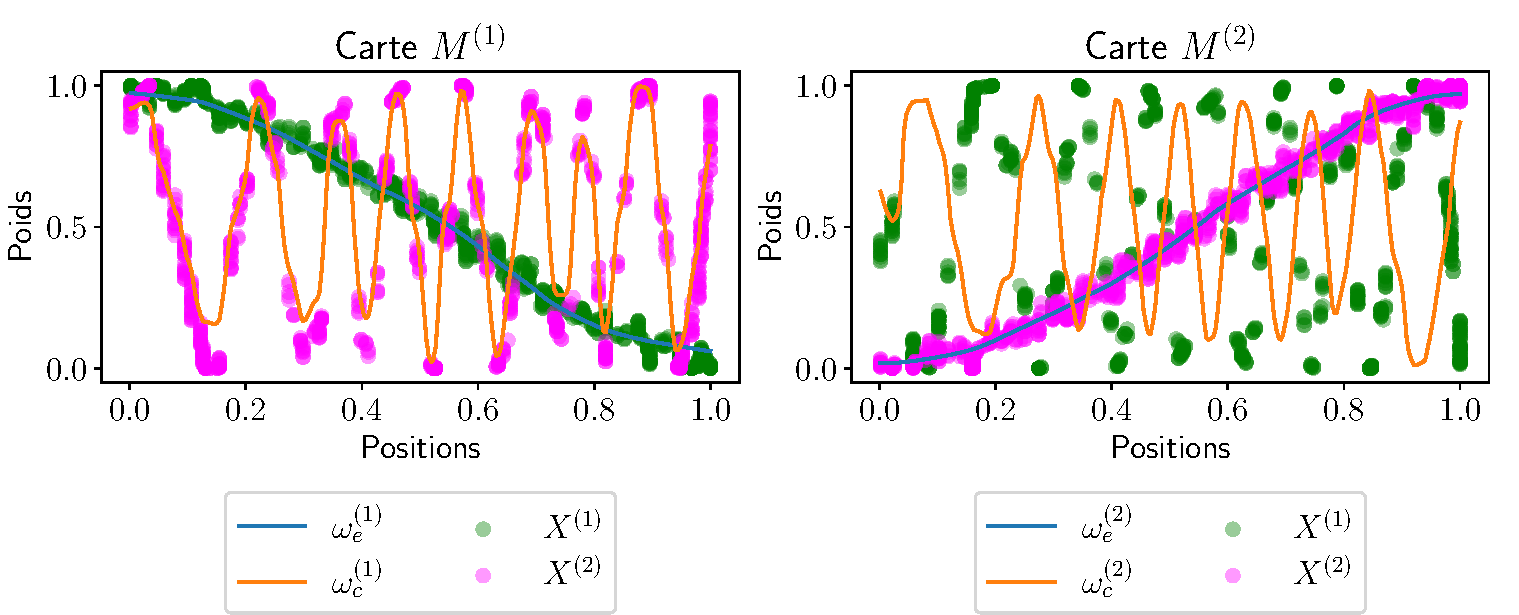
\includegraphics[width=\textwidth]{lissa/weights_19999.pdf}
	\caption{Représentation cartographique des poids et entrées pour des entrées sur une courbe de Lissajous. Les poids contextuels se disposent en zones afin de différencier les BMUs selon l'entrée externe et l'entrée contextuelle. Une zone est une carte d'une sous-region des entrées externes \label{fig:lissa}}
\end{figure}

\begin{figure}[h!]
	\centering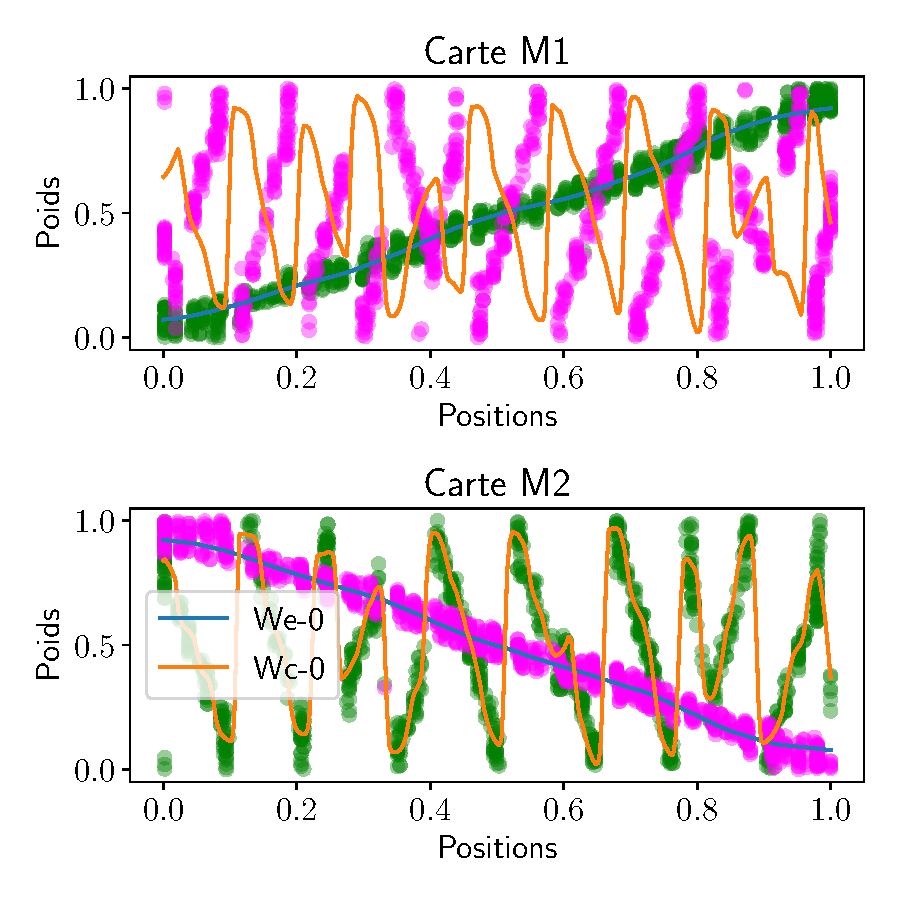
\includegraphics[width=\textwidth]{2som_square_w.pdf}
	\caption{Représentation cartographique des poids et entrées dans le patch $[0,1]^2$. Les poids contextuels s'organisent en zones qui cartographient des sous région de l'espace d'entrée. \label{fig:ind}}
\end{figure}

Dans ces deux derniers cas, les cartes présentent encore une organisation en zones des poids contextuels, tout comme le comportement observé sur le cercle. 
Le nombre de zones est similaire à ce qui est observé sur le cercle, alors que la répartition des entrées est différente. Par contre, la forme des zones varie légèrement.
Contrairement au cas précédents, les BMUs se répartissent sur toutes les valeurs de $\w_c$ dans une zone.

Nous pouvons en conclure que la présence de zones est un comportement systématique de la carte étant donné qu'elles sont observées même lorsque les entrées sont indépendantes. 
Cependant, elles émergent de l'organisation seulement lorsque qu'elles sont nécessaires, lorsqu'une carte doit pouvoir différencier au moins deux valeurs d'entrée contextuelles différentes correspondant à une même valeur d'entrée externe.
La forme des zones et la réponse des cartes dépend ensuite de la relation entre entrées. Plus

Sur la distribution indépendante, la carte ne présente pas de zone morte. La totalité d'une zone se déploie de manière à couvrir l'ensemble des valeurs de $U$ correspondant à cette zone, ce qui est également observé en figure ~\ref{fig:lissa} pour les courbes de Lissajous. Une zone agit alors comme une petite carte d'une sous-région de l'espace d'entrée. 

Nous pouvons le constater sur la Figure~\ref{fig:2som_p_d} présentant la distorsion des poids externes des cartes dans l'espace $\inpx\m{1}; \inpx\m{2}$ lorsque les entrées sont dans le carré. Les poids des cartes quantifient tout l'espace $[0,1]^2$, en notant qu'une centaine de points servent à la quantification, pour deux cartes de taille 500. La carte $M\m{1}$ parcourt l'espace selon les valeurs de $\inpx\m{1}$ tandis que $M\m{2}$ le parcours selon les valeurs de $\inpx\m{2}$.

\begin{figure}[h!]
	\begin{minipage}{0.48\textwidth}
		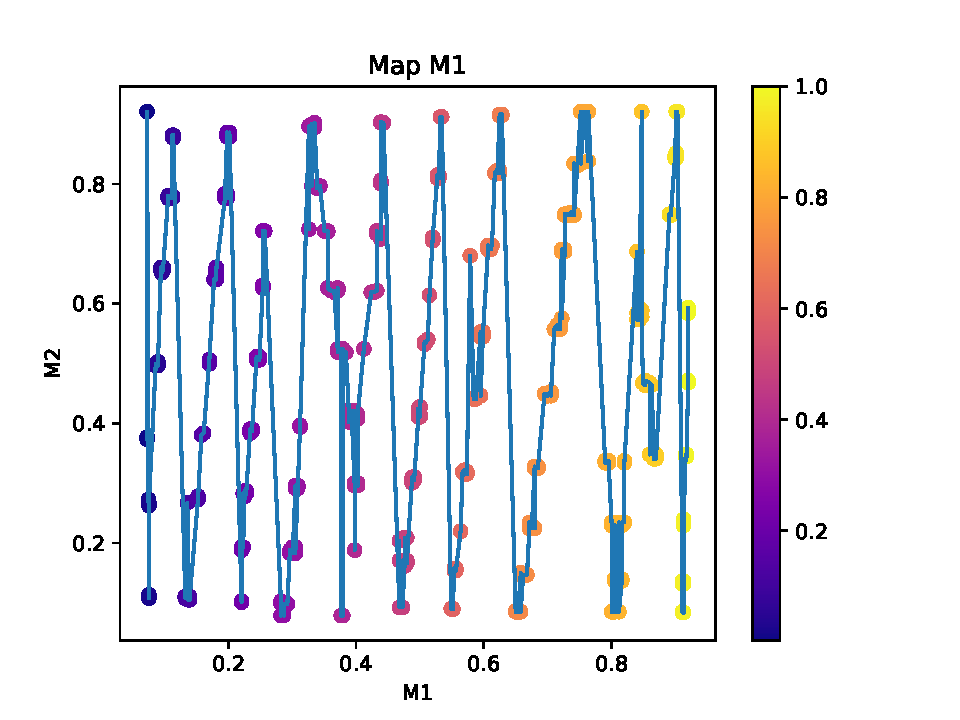
\includegraphics[width=\textwidth]{2som_square_d}
	\end{minipage}
	\begin{minipage}{0.48\textwidth}
		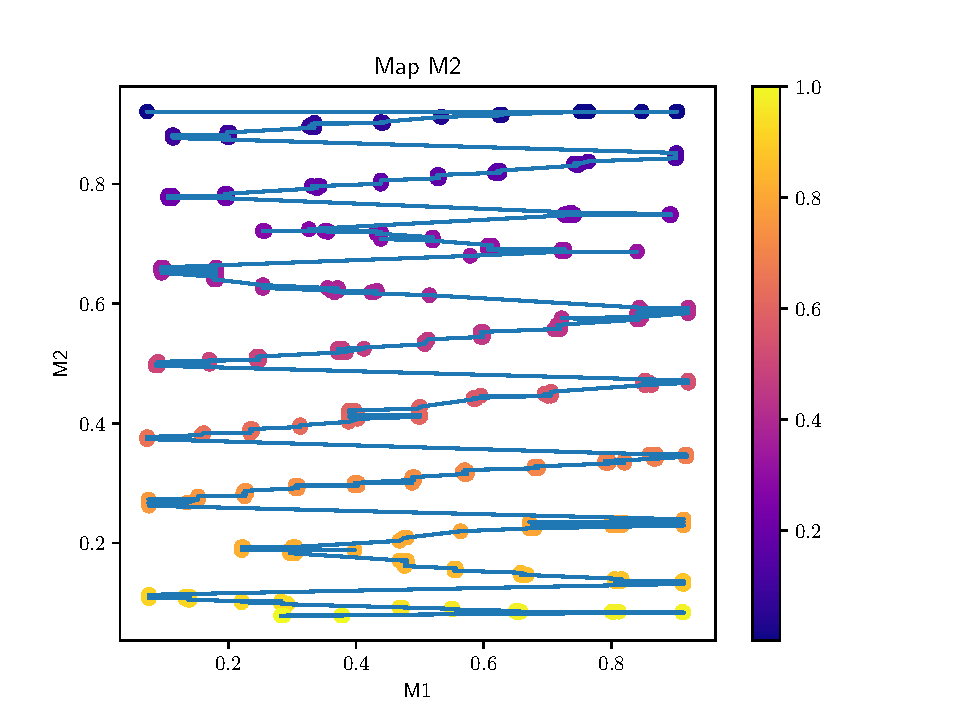
\includegraphics[width=\textwidth]{2som_square_d2}
	\end{minipage}
	\caption{Représentation de la distortion des poids des deux cartes dans l'espace d'entrée $\inpx\m{1}, \inpx\m{2}$ lorsque les entrées sont indépendantes. Les cartes s'organisent de façon à quadriller le carré, l'une selon les $\inpx\m{1}$, l'autre selon les $\inpx\m{2}$. Bien que chaque carte a 500 n\oe{}uds, on observe seulement environ 90 valeurs possibles pour les paires $\w_e(\bmu\m{1}),\w_e(\bmu\m{2})$ \label{fig:2som_p_d}}
\end{figure}


Enfin, nous voulons vérifier si les cartes sont robustes au bruit. 
Sur des données en forme d'anneau (Entrées~\textbf{(E)}), représentées en Figure~\ref{fig:anneau_w}, nous observons le même comportement que sur les courbes de Lissajous ou le carré~: le nombre de zones de poids contextuels est défini par l'organisation de la carte. Chaque zone correspond à un même intervalle de valeurs pour le couple $(\inpx, U)$.
Enfin, notons que dans toutes ces dispositions d'entrées le tracé de $U$ en fonction de la position du BMU dans chaque carte montre une relation fonctionnelle entre $U$ et les positions du BMU, ce qui montre que chaque carte de l'architecture a appris une représentation du modèle d'entrée. Nous reviendrons plus en détail sur l'utilisation de $U$ dans l'analyse des réponses des cartes au chapitre \ref{chap:indicateur}.


\begin{figure}[h!]
	\centering\includegraphics[width=\textwidth]{anneau/weights.pdf}
	\caption{Représentation cartographique des poids et entrées pour des entrées sur un anneau. \label{fig:anneau_w}}
\end{figure}

\subsection{Mécanismes de formation des zones de poids contextuels}

Nous avons observé sur ces distributions d'entrées en 2D les comportements suivants qui vérifient et complètent les hypothèses formulées sur la disposition d'entrées en cercle.
Tout d'abord, la quantification vectorielle reste correctement réalisées sur les différentes dispositions d'entrées. 
Les valeurs prises par les poids sont disposées en étages du fait des zones.
Cette organisation en zones intervient dès que la disposition des entrées implique d'avoir à séparer au moins deux valeurs de $U$ pour une même entrée externe.
Le fait que des zones existent n'implique pas la détection d'une relation entre entrées~: la carte forme des zones lorsque les entrées sont indépendantes. Cette formation de zones est systémique aux mécanismes d'auto-organisation des cartes. Le nombre de zones ne varie pas en fonction des distributions d'entrées. Cela implique que les mécanismes d'évolution de la carte conduisent systématiquement à la formation des zones, et que l'organisation s'adapte ensuite à cette disposition. 

\subsubsection{Dépendance aux paramètres des cartes}

La formation de zones dépend notamment des valeurs des rayons externes et contextuels. 
En effet, $r_c \geq r_e$, la carte ne s'organise pas en zones. La formation de celles-ci intervient pour $r_c << r_e$. Sur le modèle d'entrée en cercle, elles sont observées à partir de $r_c = \frac{1}{3} r_e$.
Ces zones apparaissent grâce au fait que la proximité des poids externes est priorisée par rapport aux poids contextuels par le grand rayon de voisinage externe. 
Ce rapport introduit une relation subordonnée entre les poids. 
Il semble que le nombre de zones dépend en partie du rapport entre $r_c$ et $r_e$. Une étude plus approfondie devrait être réalisée pour analyser l'influence des paramètres sur l'organisation. 
L'organisation au sein d'une zone et la forme des poids contextuels dépendent par contre du modèle d'entrées.

\subsubsection{Influence de la présence de zones sur la recherche de BMU par relaxation}

Nous nous intéressons au passage à l'influence de la formation de zones sur le processus de relaxation.
Nous pourrions penser que ces zones favorisent la recherche de consensus lors de la relaxation et la convergence des poids.
Nous traçons en figure~\ref{fig:conv_rcre} le nombre de pas moyen nécessaire à la recherche du BMU par relaxation et les indicateurs de convergence des poids des cartes.
Ces valeurs sont similaires dans les cas d'une carte formant des zones et d'une carte n'ayant pas formé de zones. Sur des cartes 1D, nous n'observons donc pas d'amélioration de la relaxation grâce à la formation de zones.
Cela montre cependant que la convergence de la relaxation n'est pas spécifique aux valeurs de paramètres choisies dans ces expériences et est ainsi une méthode générale de connexion entre cartes.


\begin{figure}[h!]
	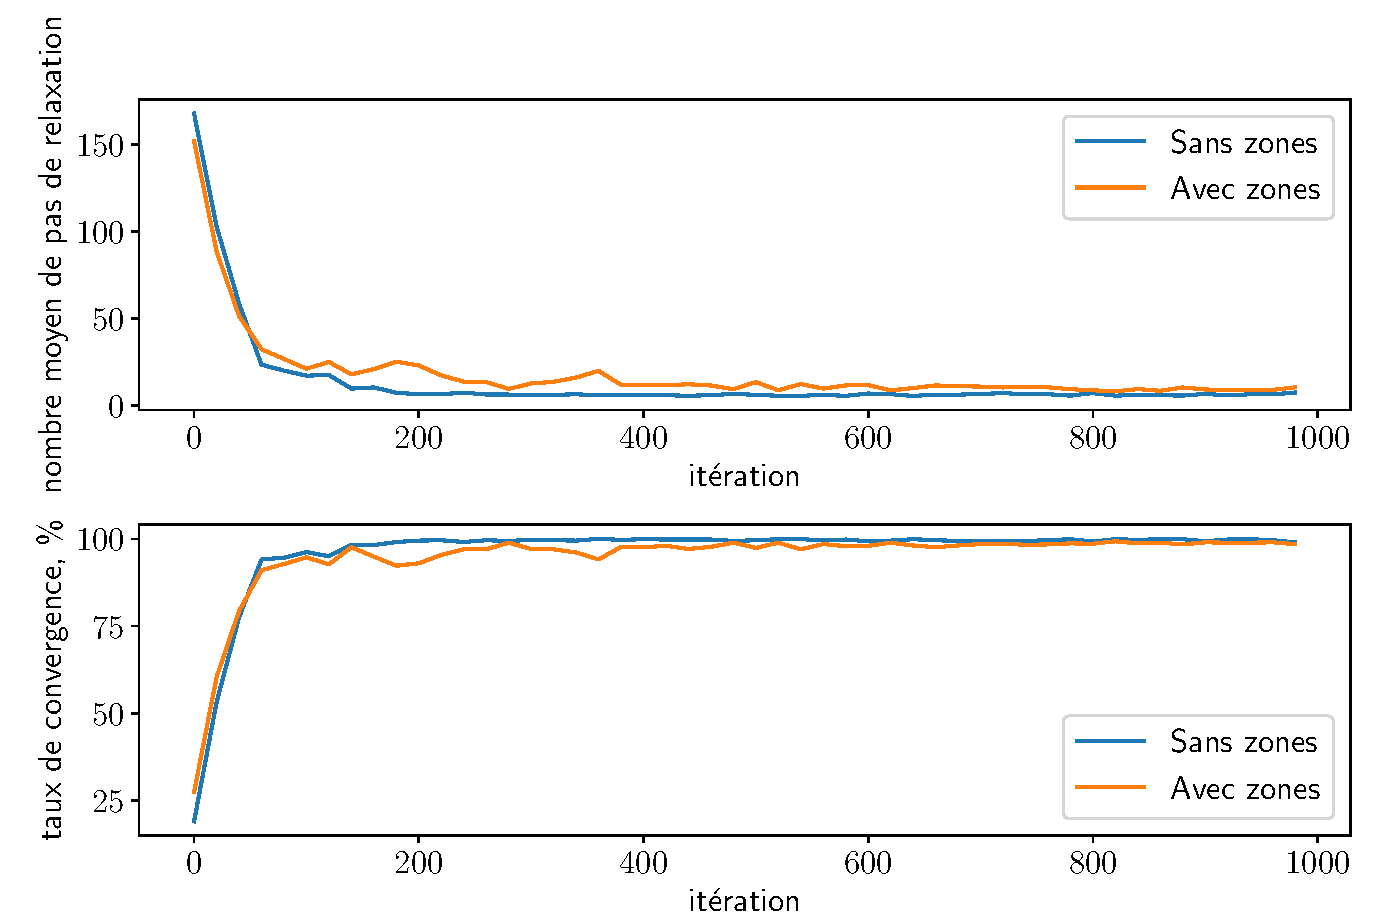
\includegraphics[width=\textwidth]{rceqre/convergence_relax.pdf}
	\caption{\'Evolution du nombre moyen de pas de relaxation et du taux de convergence pour une organisation de cartes ayant formé des zones de poids contextuels ($\frac{r_e}{r_c} = 10$ ) et une organisation n'ayant pas formé de zones ($\frac{r_e}{r_c} = 1$). Dans les deux cas, la relaxation mène à un consensus. 
	Donc, dans des cartes en une dimension, la formation de zones ne favorise pas significativement la convergence de la relaxation. Par ailleurs, le mécanisme de relaxation a donc un sens général, quels que soient les paramètres des cartes \label{fig:conv_rcre}}
\end{figure}

\subsubsection{Discussion}

Au sein d'une même zone, dans laquelle les poids externes ont des valeurs très proches, les poids contextuels s'organisent de manière à former une sous-carte des valeurs possibles de l'entrée contextuelle.
On pourrait donc introduire une notion d'indices primaires et secondaires, l'indice primaire étant celui de la zone et l'indice secondaire la position dans la zone.
Cette notion d'indices primaires et secondaires est également observée dans le cerveau, proposé en 1986 par \cite{ballard_cortical_1986}. Les neurones du cortex V1, par exemple, gèrent leurs connexions et leur organisation comme schématisé en figure~\ref{fig:ballard}.
Les neurones situés à différents emplacements sur cortex V1 ne reçoivent pas la même partie de l'entrée visuelle. Ces entrées différenciées forment une indexation~\emph{primaire} de V1. Au sein d'une zone de même indice primaire, les neurones s'organisent de façon à représenter tout le sous-espace des entrées ayant été présenté à la zone. Cette sous-carte définit alors des indices secondaires.
Ici, la même entrée est certes présentée à toute la carte, donc la proximité avec le modèle biologique est limitée.

D'un point de vue computationnel, l'organisation d'une carte encode finalement une méthode de modulation~: la valeur de l'activité externe est modulée par une activité contextuelle alternant des valeurs hautes et basses. Cette modulation permet ainsi d'encoder en une seule valeur $X$ et $U$, le modèle d'entrée. Cette modulation émerge de la dynamique d'apprentissage des cartes. Cette méthode de modulation rejoint des méthodes traditionnellement utilisées en apprentissage automatique.
Les zones forment ainsi un deuxième niveau de quantification vectorielle, moins précis que le premier, mais qui encode la valeur de $U$ et non seulement de l'entrée $X$. 
Ce deuxième niveau de quantification vectorielle encode l'information sur $U$ dans chaque carte et nous permet l'utilisation de l'architecture comme prédiction d'une entrée manquante.

\begin{figure}[h!]
	\centering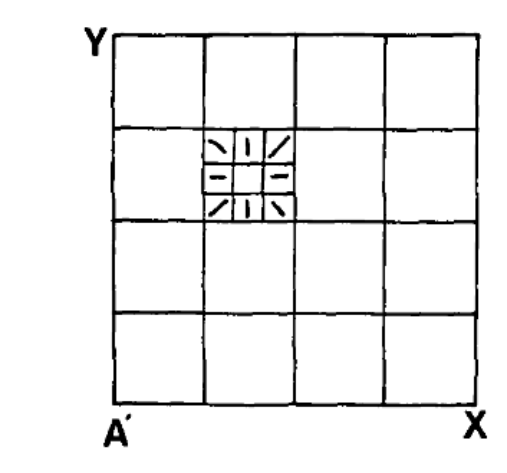
\includegraphics[width=0.4\textwidth]{ballard_primary_secondary.png}
	\caption{Schématisation d'une répartition en indices primaires et secondaire des neurones d'une aire corticale, tirée de~\cite{ballard_cortical_1986}. 
	Les auteurs observent que la réponse de neurones du cortex est organisée en zones selon leur position, formant des indices primaires. Les carrés de la figure représentent cette première indexation.
	Ces zones reçoivent différentes portions de l'espace d'entrée~: les zones situées à gauche du cortex traitent les signaux venant du champ visuel de gauche et ainsi de suite pour couvrir tout le champ visuel.
	Au sein d'une zone, les neurones cartographient toutes les valeurs possibles de l'entrée sous forme de carte topologiquement ordonnée, formant une indexation secondaire. \label{fig:ballard}}
\end{figure}

\section{Prédiction d'entrée dans des architectures de trois cartes 1D}

% L'observation des mécanismes d'organisation à l'\oe{}uvre dans des architectures de deux cartes nous confirme que le modèle d'entrées est bien appris dans chacune des cartes de l'architecture grâce aux connexions entre cartes.
% Nous utilisons maintenant le fait qu'une architecture ait appris le modèle dans une tâche de prédiction d'entrée.

% Cette utilisation en tant que prédiction a certes une valeur applicative, car il s'agit d'un cas d'utilisation possible d'une architecture CxSOM pour une tâche de mémoire associative. Néanmoins, la prédiction permet avant tout de valider l'apprentissage du modèle par l'architecture d'un point de vue d'une carte. Par exemple, dans le cas de données réelles, le modèle d'entrée n'est pas forcément connu. 
% La prédiction permet alors de valider l'apprentissage du modèle~: étant donné un modèle d'entrées dans lequel la connaissance de deux entrées et du modèle détermine la valeur de la troisième entrée~; si l'architecture de cartes, à partir de ces deux entrées est capable de prédire la valeur de la troisième entrée, alors nous pouvons conclure que l'architecture a bien appris les relations entre entrées.
Nous cherchons maintenant à utiliser l'apprentissage du modèle d'entrée dans une tâche de prédiction. Cette utilisation permettra de valider l'apprentissage du modèle par l'architecture. \'Etant donné un modèle d'entrées dans lequel la connaissance de deux entrées et du modèle détermine la valeur de la troisième entrée~; si l'architecture de cartes, à partir de ces deux entrées est capable de prédire la valeur de la troisième entrée, alors nous pouvons conclure que l'architecture a bien appris les relations entre entrées. 
Nous utiliserons ensuite cette capacité de prédiction sur des entrées réelles pour le contrôle d'un drone.

\subsection{Architecture de trois cartes et modèle d'entrées utilisé}

Nous testons d'abord la qualité de la prédiction sur des dispositions d'entrées jouet.
Pour qu'une carte puisse faire une prédiction correcte, nous choisissons des dispositions d'entrées telles que la connaissance des entrées et du modèle détermine l'entrée manquante.
Nous prendrons ainsi deux moèdles d'exemple~: des entrées disposées sur un cercle en deux dimensions plongé et pivoté dans l'espace en 3D (Entrées \textbf{H}) ainsi que sur un plan pivoté en trois dimensions (Entrées \textbf{G}). Ces entrées sont tracées en figure~\ref{fig:inputs_3D}. Dans les deux cas, la connaissance de deux des trois coordonnées et du modèle d'entrée permet de déterminer la troisième avec précision.

Ces tâches de prédiction sont réalisées sur une architecture de trois cartes 1D, toutes connectées entre elles. 
Chaque carte prend donc deux entrées contextuelles, les positions des BMUs des deux cartes voisines, et de ce fait possède deux couches contextuelles $\w_{c_0}$ et $\w_{c_1}$.

L'algorithme de prédiction est présenté en Figure~\ref{fig:schema_pred}. Celle-ci peut être directement réalisée par les règles d'évolution du modèle CxSOM sans modification majeure.
Nous effectuons l'apprentissage des cartes lors d'une première phase.
Ensuite, nous choisissons une des cartes $M\m{p}$ comme carte prédictive. Lors de la phase de prédiction, cette carte ne reçoit plus son entrée externe, mais seulement ses entrées contextuelles. 
Les autres cartes reçoivent toutes leurs entrées.
La phase de prédiction est une phase de test durant laquelle les poids de toutes les cartes ne sont pas mis à jour. Les règles de calcul et paramètres sont conservés entre apprentissage et prédiction.
La carte prédictive $M\m{p}$ prend comme activité globale seulement son activité contextuelle, c'est-à-dire la moyenne des deux activités contextuelles. Le principe de relaxation ne change pas par rapport à l'apprentissage.
Nous choisissons comme valeur de prédiction le poids externe du BMU de la carte prédictive $\w\ext\m{p}(\bmu\m{p})$. 
Ce est choisi uniquement grâce aux entrées contextuelles de la carte $M\m{p}$. 
Nous vérifierons si cette prédiction est proche de l'entrée théorique $\inpx\m{p}$, qui n'a pas été présentée à la carte.

\begin{figure}
	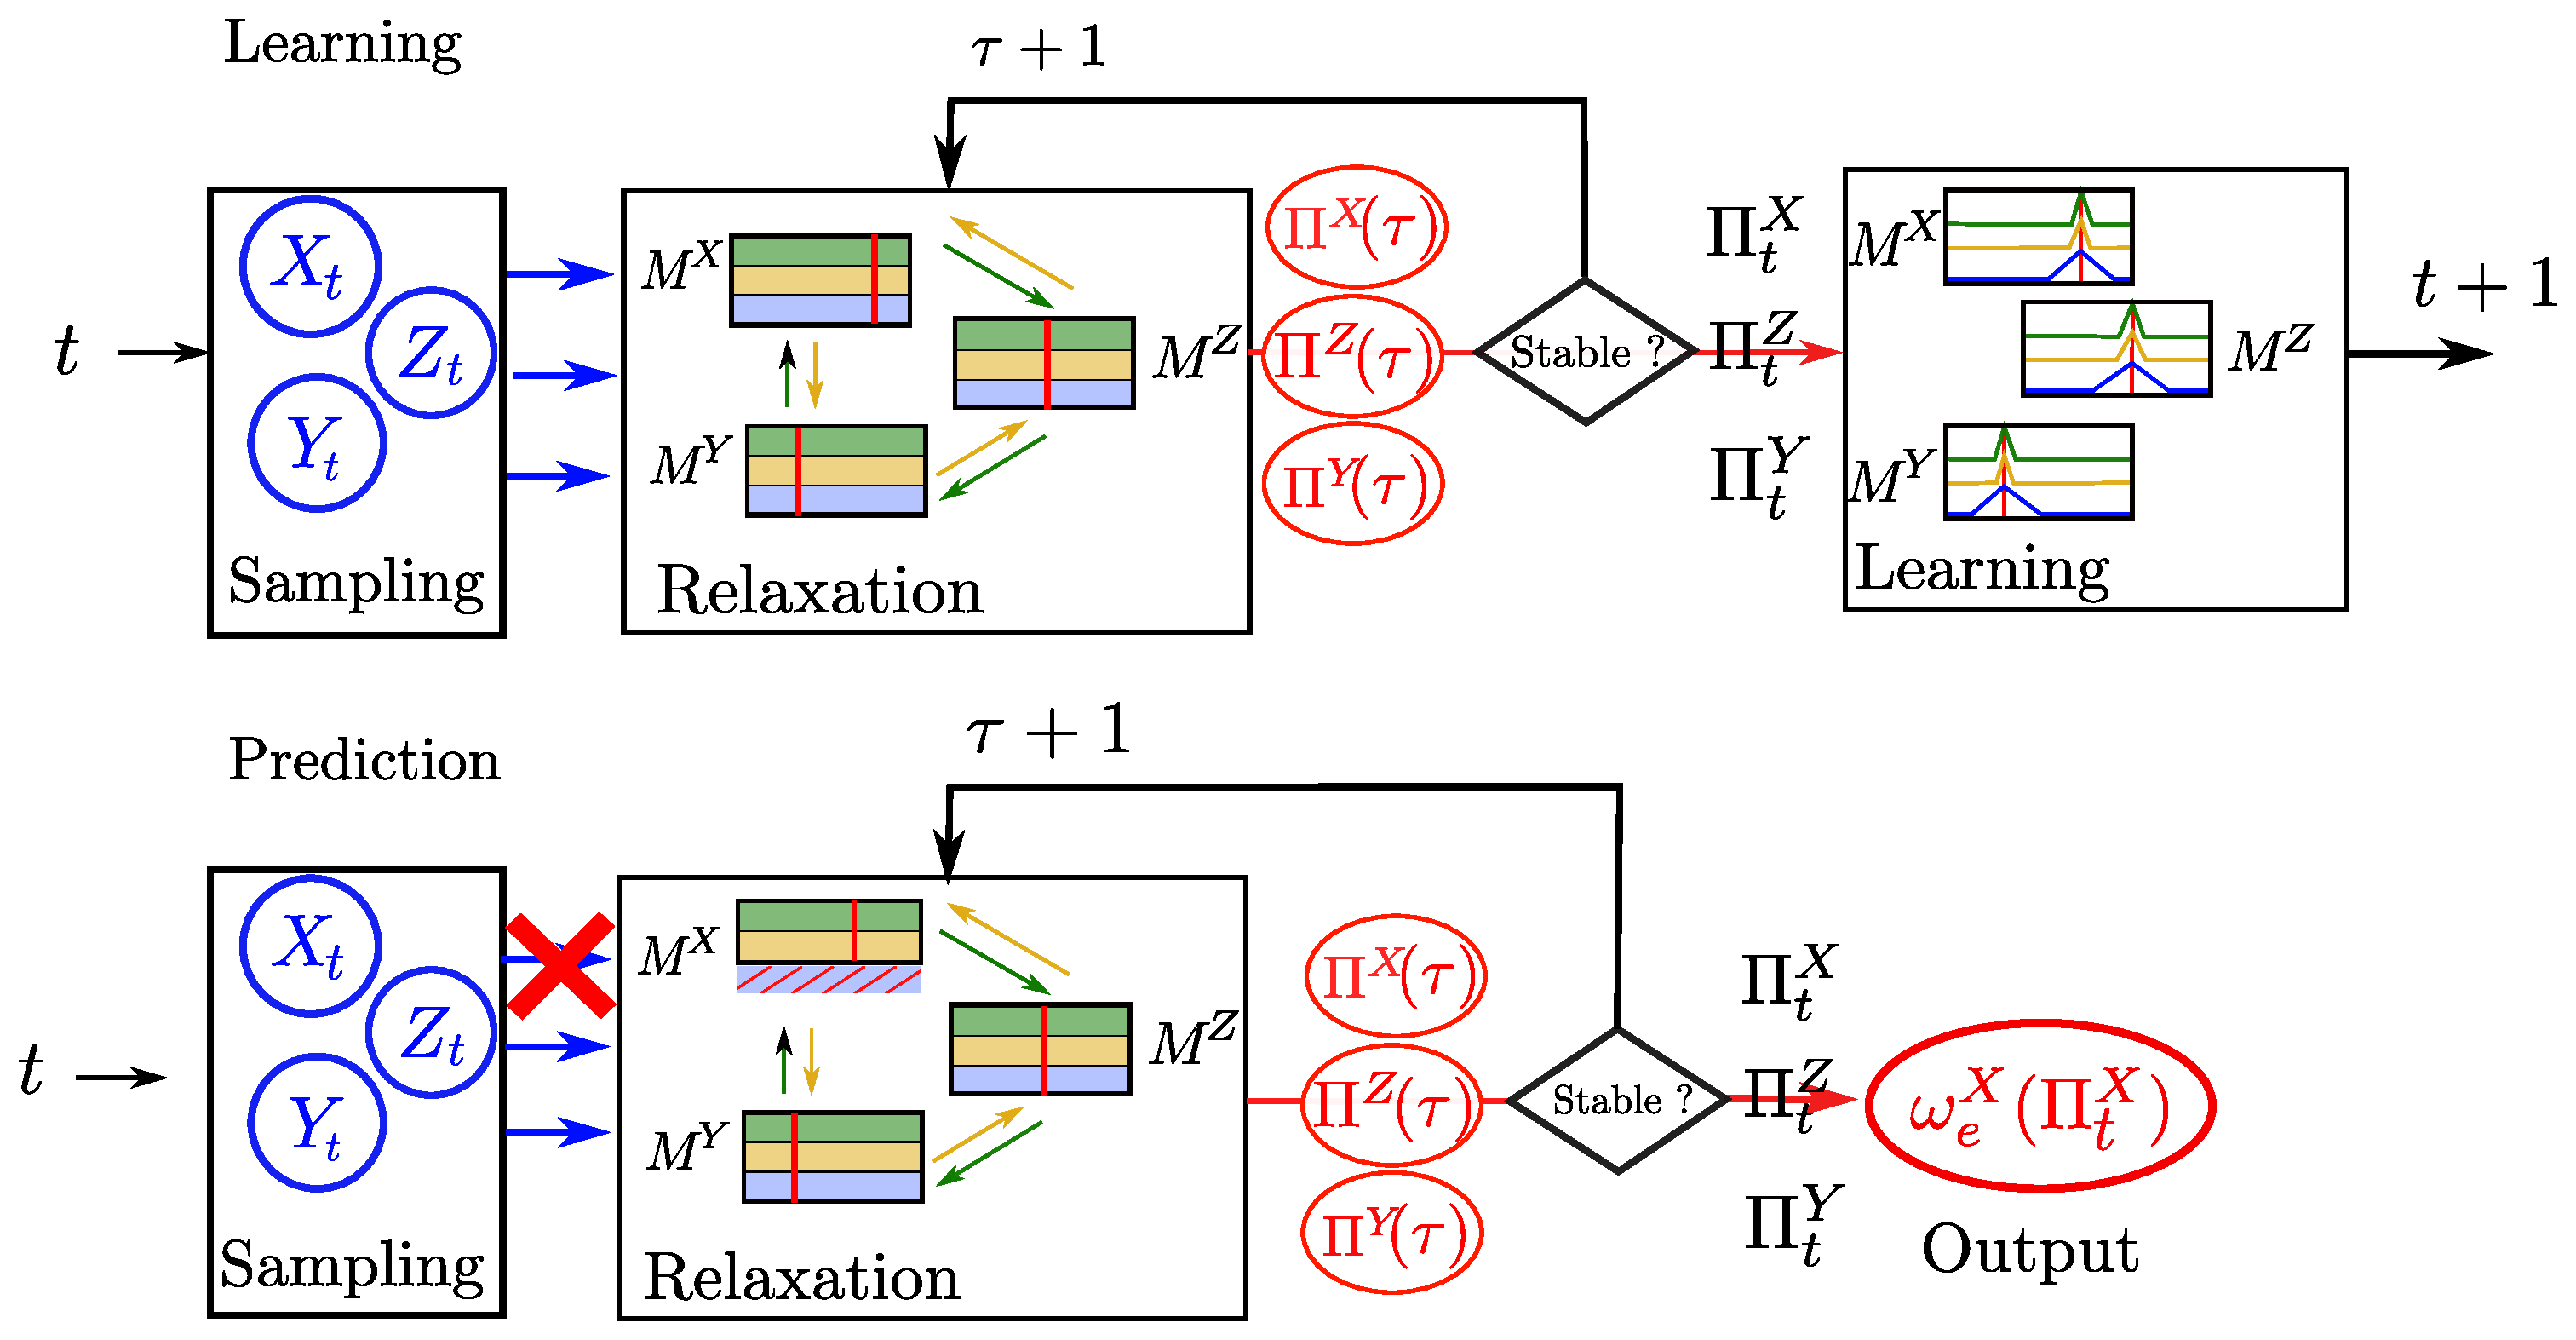
\includegraphics[width=\textwidth]{learning_tests.pdf}
	\caption{Schéma descriptif des opérations effectuées lors de l'apprentissage et de la phase de prédiction.\label{fig:schema_pred}}
\end{figure}

\subsection{Résultats}

La figure \ref{fig:w_cercle} présente la disposition des poids des trois cartes de l'architecture après apprentissage ainsi que des entrées associées. Comme dans la version à deux cartes, les poids contextuels s'organisent en plusieurs zones au sein desquelles la valeur de $U$ est située dans une même plage de valeur.
Nous pouvons remarquer que les deux couches de poids contextuels forment les mêmes zones. Le nombre de zones est équivalent à celui observé pour l'architecture de deux cartes.
La figure \ref{fig:pred_cercle} présente ensuite l'erreur obtenue lors de la phase de prédiction. 
Ici, l'entrée $X\m{1}$ n'est ici pas présentée à la carte et sa valeur est prédite par $\w\ext\m{1}{\bmu\m{1}}$. 
Cette figure nous montre que la prédiction est correctement réalisée par l'architecture de cartes. Remarquons que la disposition de l'erreur en lignes horizontales correspond aux zones définies par les valeurs des poids contextuels d'une carte.

\begin{figure}[h!]
	\centering\includegraphics[width=\textwidth]{cercle3D/weights.pdf}
	\caption{Représentation cartographique des poids et entrées dans l'architecture de trois cartes apprenant sur un cercle en trois dimensions. Nous observons la formation de zones similaires au cas en deux dimensions. \label{fig:w_cercle}}
\end{figure}

\begin{figure}[h!]
	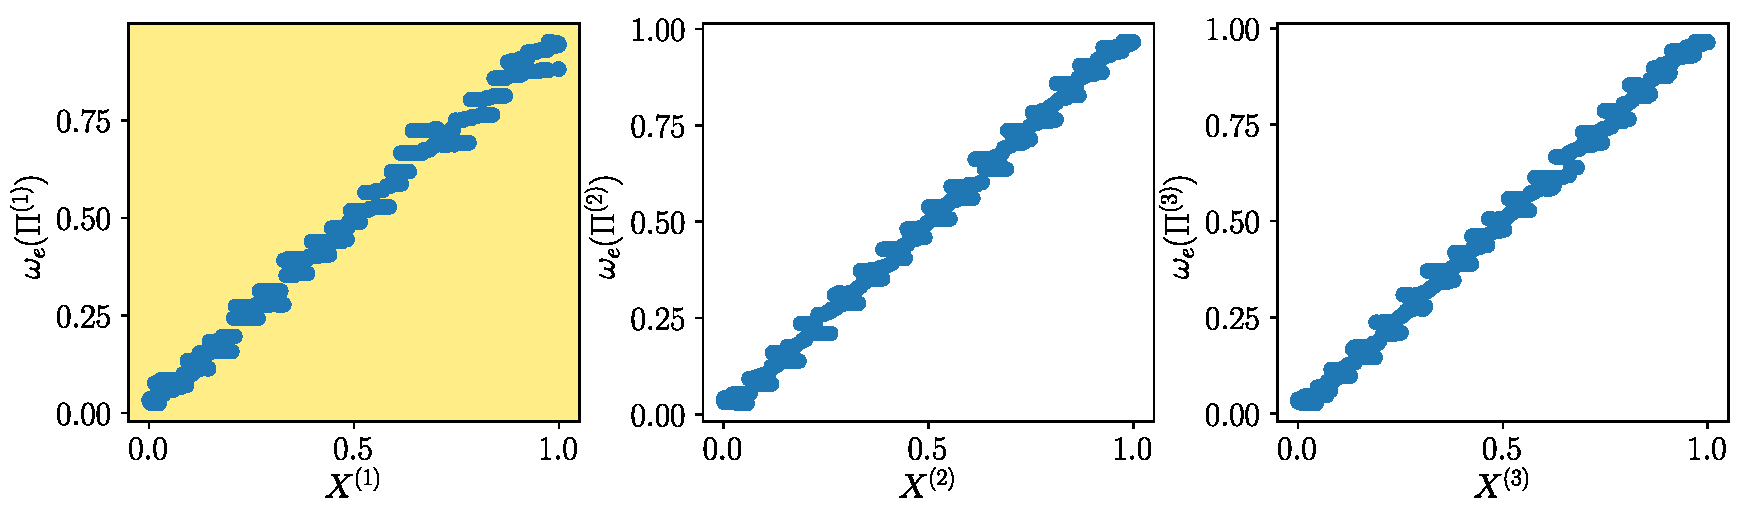
\includegraphics[width=\textwidth]{cercle3D/error-closed.pdf}
	\caption{Erreur de prédiction de $\inpx\m{1}$ par $\w_e(\bmu\m{1})$ lorsque les entrées sont sur un cercle en trois dimensions. $\inpx\m{1}$ n'a pas été présenté à $M\m{1}$.
	 Les nuages de points correspondant à $M\m{2}$ et $M\m{3}$ correspondent à l'erreur de quantification dans les cartes 2 et 3 qui ont reçu leur entrée externe. Ces tracés montrent une bonne prédiction de $\inpx\m{1}$ par la carte 1. \label{fig:pred_cercle}}
\end{figure}


Nous traçons également en Figure~\ref{fig:plan3} la disposition des cartes et l'erreur de prédiction obtenue pour des entrées située sur un plan 2D de l'espace en trois dimensions.
Ici encore, La connaissance de $X\m{2}$ et $X\m{3}$ définit bien une seule valeur possible de $X\m{1}$. 
La prédiction est bien réalisée, en remarquant une erreur assez élevée. 
Nous avons vu que les poids externes des cartes s'étalaient sur le plan en discrétisant l'espace en une centaine de points seulement, bien que chaque carte soit de taille 500 (Voir Figure~\ref{fig:2som_p_d}). 
Cette discrétisation se retrouve dans l'erreur de prédiction pour trois cartes.
Cette capacité de prédiction est peu précise, mais il s'agit d'une prise de décision induite par l'auto-organisation des cartes.

\begin{figure}[h!]
	\begin{minipage}{0.48\textwidth}
	\centering\includegraphics[width=\textwidth]{plan/weights}
	\end{minipage}
	\begin{minipage}{0.48\textwidth}
	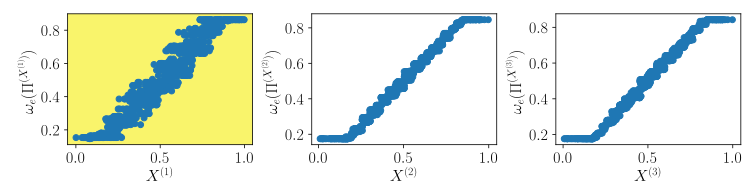
\includegraphics[width=\textwidth]{plan/zclosed-1-19999_error}	
	\end{minipage}	
	\caption{Représentation cartographique des poids et entrées des trois cartes après apprentissage d'un plan pivoté en 3D et erreur de prédiction. 
	Le découpage de l'espace par les cartes permet de prédire correctement une entrée. La précision faible de la quantification au niveau des zones explique l'erreur de prédiction moins précise dans ce cas. \label{fig:plan3}}
	\end{figure}


Nous nous intéressons enfin à l'influence de l'organisation en zones de poids sur la capacité de prédiction.
Nous effectuons pour cela pour une phase apprentissage et prédiction sur une architecture dans laquelle $r_c = r_e$. Nous avions en effet vu que ce choix de paramètres n'engendre pas la formation de zones.
Aucune prédiction n'est réalisée. 
Dans cette situation, les cartes sont \og organisées \fg{} dans le sens ou les poids externes et contextuels ont évolué vers un état stable et présentent une continuité. Les BMUs sont choisis par relaxation, donc en fonction de toutes les cartes de l'architecture. Nous ne pouvons cependant pas parler d'un apprentissage associatif car les cartes ne sont pas capable d'utiliser les relations. Les zones permettent donc aux cartes d'encoder les relations entre entrées et de les réutiliser en sortie.

% Lorsqu'il manque des informations pour prédire correctement l'entrée, par exemple dans le cas du cercle en deux dimensions et d'une architecture de deux cartes, l'activation est cohérente. Si on ne présente pas l'entrée $\inpx\m{2}$ à la carte $M\m{2}$, deux bulles d'activité se formeront aux deux emplacements possibles pour $\bmu\m{2}$, sans qu'une des deux options ne soit systématiquement privilégiée par l'architecture.


\begin{figure}[h!]
	\centering\includegraphics[width=0.9\textwidth]{rceqre/prediction.pdf}
	\caption{Prédiction de l'entrée $X\m{1}$ lorsque $r_c = r_e$. La prédiction n'est pas effectuée. Ainsi, sans formation de zones, la capacité de prise de décision n'est plus réalisable par une carte de l'architecture. \label{fig:rcre_pred}}
\end{figure}
	

\section{Influence des connexions et des paramètres}

Dans toutes les expériences précédentes, nous avons utilisé une architecture de cartes toutes connectées. Nous présentons maintenant quelques observations ouvrant des questions sur l'influence des connexions dans une architecture.

Nous nous intéressons tout d'abord à des grandes architectures de cartes. Nous avons vu qu'une architecture de deux cartes apprenant le carré $[0,1]^2$ se déplie de manière à former deux indices. Nous pouvons effectuer la même expérience pour une architecture de $K$ cartes apprenant sur tout l'espace $[0,1]^K$, toutes connectées.
La figure \ref{fig:bigdim} présente la forme des poids d'un telle disposition, sur une architecture de 10 cartes toutes connectées. Les entrées sont tirées dans le cube $[0,1]^9$, et les entrées $\inpx\m{9}$ et $\inpx\m{10}$ sont identiques.
Nous remarquons que les poids contextuels tendent vers une valeur moyenne de 0.5 dans chaque carte lorsque les entrées sont indépendantes. L'architecture équivaut donc à 9 cartes indépendantes, ce qui est logique par rapport à la disposition des entrées qui sont ici toutes indépendantes. Par contre, les poids contextuels correspondant aux entrées identiques se déplient totalement, comme en figure~\ref{fig:id_results}. La prédiction de l'entrée $9$ est bien réalisée lorsque la carte ne reçoit pas l'entrée. Ainsi, il semble que les connexions correspondant à des entrées indépendantes finissent par se moyenner pour ne plus jouer dans l'apprentissage des connexions correspondant à des entrées dépendantes et ne polluent donc pas l'apprentissage des relations.
Cette expérience mérite d'être étudiée plus en détail pour plus de types de connexions entre entrées. 
En particulier, on peut se demander si le comportement de l'architecture sur des entrées en grande dimension permet d'extraire automatiquement des relations entre entrées, ce qui serait un comportement émergeant d'un grand nombre d'interactions.

\begin{figure}[h!]
	\begin{minipage}{\textwidth}
	\includegraphics[width=\textwidth]{bigdim/weights.pdf}
	\end{minipage}
\begin{minipage}{\textwidth}
	\centering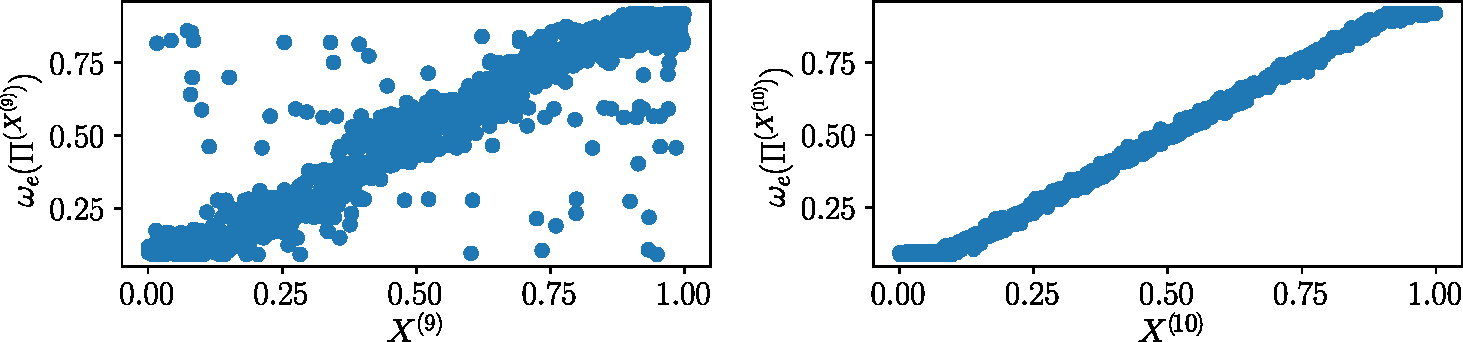
\includegraphics[width=0.8\textwidth]{bigdim/error_closed.pdf}
	\caption{En haut, tracé des poids des cartes pour une architecture de 10 cartes toutes connectées. Nous avons ici seulement tracé 4 cartes sur les 10. Les entrées sont indépendantes, sauf les entrées $\inpx\m{9}$ et $\inpx\m{10}$ qui sont identiques. Nous remarquons que les poids contextuels se moyennent autour de 0.5, sauf ceux correspondant aux entrées dépendantes. En pas, nous traçons l'erreur de prédiction de la carte 9 lorsqu'elle ne reçoit pas d'entrée. La prédiction est bien réalisée~: les connexions contextuelles inutiles ne polluent pas l'apprentissage. \label{fig:bigdim}}
\end{minipage}
\end{figure}

Dans une deuxième expérience, nous reprenons en entrée le cercle tourné en trois dimensions (\textbf{G)}. Nous comparons le comportement d'une architecture de trois cartes connectées réciproquement présenté plus haut, à celui d'une architecture de trois cartes connectées en boucle : $M\m{1}$ est connectées à $M\m{2}$, connectée à $M\m{3}$, connectée à $M\m{1}$. 
La phase d'apprentissage forme des motifs similaires à ceux observés sur la disposition avec rétroactions. Les poids contextuels forment des zones et $U$ est une fonction du BMU dans chaque carte. 
Cependant, lorsque nous effectuons la phase de prédiction,la carte $M\m{1}$ ne reçoit plus d'entrée externe et son activité contextuelle, relative à une seule couche de poids, dépend donc seulement de $M\m{3}$. La carte $M\m{2}$ intervient seulement via l'activité de cette dernière carte.
Nous observons que la prédiction est moins précise que dans l'architecture avec rétroaction, mais est globalement réalisée. Des connexions distantes influencent donc une carte de manière moindre. L'influence des connexions sera à réaliser pour un passage sur une grande architecture.

\begin{figure}[h!]
	\begin{minipage}{\textwidth}
		\centering\includegraphics[width=\textwidth]{loop/weights.pdf}
	\end{minipage}
	\begin{minipage}{\textwidth}
		\centering\includegraphics[width=\textwidth]{loop/prediction.pdf}
		\caption{Poids à l'issue de l'apprentissage et erreur de prédiction de $\inpx\m{1}$ dans une architecture de 3 cartes connectées en boucle. Bien que les poids s'organisent de façon similaire aux expériences dans lesquelles les cartes sont connectées réciproquement, la prédiction est moins bien réalisée. L'influence des connexions diminue donc rapidement avec la distance dans l'architecture, mais reste présente.\label{fig:3som_loop}}
	\end{minipage}
\end{figure}

	
\section{Prédiction d'entrée réelles~: application au contrôle d'un drone}

Nous avons vu une possibilité d'application d'une architecture CxSOM dans une tâche de prédiction d'entrée. Nous sortons du cadre des entrées simulées pour nous placer dans un cas de contrôle réel. 
Nous disposons d'un drone quadricoptère, contrôlé à distance par ordinateur via le logiciel ROS.
Ce drone possède une caméra frontale ainsi qu'un ensemble de capteurs internes. Chacun de ces capteurs peut être considéré comme une modalité d'un espace multimodal. 
La commande envoyée au drone à chaque instant est également une modalité de l'environnement.

Le principe de cette expérience est d'apprendre, à l'aide d'une architecture de cartes, les relations existant entre les modalités des capteurs et de la commande. Dans un deuxième temps, nous utiliserons les poids appris afin prédire la commande à envoyer à partir des valeurs des capteurs, en temps réel sur une trajectoire du drone.
Afin que les relations entre la commande et les capteurs soient significatives, nous nous plaçons dans un cas d'application particulier~: le drone vole dans un couloir droit et étroit. Le but du contrôle par l'architecture de cartes est de corriger la trajectoire du drone en temps réel afin qu'il vole au milieu du couloir et ne touche pas les murs.

Lors des expériences jouets, les données étaient peu bruitées et nous nous étions assurés que chaque modalité contribuait à l'apprentissage du modèle. 
Dans cette application, les relations entre entrées sont simples, mais les données sont très bruitées. Par ailleurs, certaines entrées ne donnent pas d'information sur la valeur de la commande et peuvent polluer l'apprentissage.
Nous évaluerons grâce à cette expérience la robustesse de l'algorithme à des données bruitées et la capacité de CxSOM à réagir en temps réel malgré les étapes de relaxation.

\subsection{Méthode expérimentale}

Le drone utilisé pour l'expérience est un quadricoptère. Il possède une caméra frontale.
Nous le contrôlons à distance par un ordinateur. 
Nous plaçons le drone dans un couloir en ligne droite. Le but du contrôle est de rectifier la trajectoire à chaque instant afin que le drone vole dans le couloir sans toucher les murs. L'objectif de l'expérience est d'apprendre les relations entre les valeurs des capteurs et les commandes à l'aide d'une architecture CxSOM afin de prédire la commande lors d'une phase de test.

La commande du drone est réalisée en définissant à tout instant un angle de rotation autour de chaque axe. 
L'angle autour de l'axe $z$, $\w$ contrôle la vitesse de rotation angulaire du drône autour de cet axe. L'angle autour de l'axe $y$ contrôle la vitesse de rotation haut/bas. Enfin, l'angle autour de $x$, $\rho$, influence l'\emph{accélération} du drone selon $y$.
Dans le cadre de l'expérience, nous contrôlerons uniquement $\rho$. L'angle $\omega$ est contrôlé à l'aide d'un PID de façon à ce que la caméra du drone reste fixée au milieu du couloir, et l'angle en $y$ est maintenu à 0, de façon à ce que le drone se déplace à une altitude constante.

Les modalités présentées à l'architecture sont la commande $\rho$ et trois éléments extraits des capteurs du drone relatifs à sa position par rapport au couloir.
Nous extrayons deux éléments visuels spécifiques au couloir à partir de la caméra du drone~: l'abscisse du point de fuite du couloir $x$ et la différence entre les angles des lignes du couloir, notée $\varphi$.
Ces valeurs sont illustrées en figure~\ref{fig:drone}.
Enfin, les capteurs internes nous permettent de récupérer les vitesses linéaires $v_x,v_y,v_z$ à chaque instant selon chaque axe de déplacement. Comme nous contrôlerons l'accélération selon $y$, nous nous intéresserons à la vitesse linéaire en $y$ en tant que modalité.

Nous utilisons ainsi quatre modalités lors du déplacement du drone~: $x$, $\varphi$, $\rho$ et $v_y$.
Nous construisons une architecture CxSOM sur ces quatre modalités, composée de quatre cartes connectées chacune aux trois autres, tracée en figure~\ref{fig:archi_drone}. Chaque carte prend une des modalités comme entrée externe.


\begin{figure}
	\centering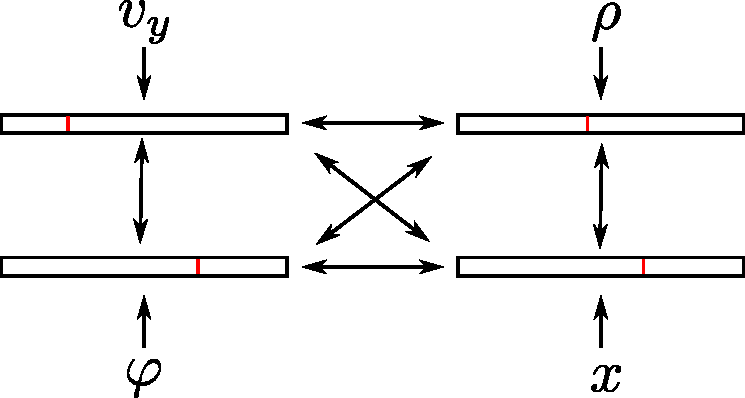
\includegraphics[width=0.5\textwidth]{archi_drone.pdf}
	\caption{Architecture de quatre cartes utilisée dans l'expérience. Chaque carte prend une modalité en entrée externe lors de l'apprentissage~: $v_y,\rho,\varphi,x$. Lors de la phase de prédiction, l'entrée $\rho$ n'est plus présentée à l'architecture et la commande envoyée au drône est $\w_e\m{\rho}(\bmu\m{\rho})$\label{fig:archi_drone}}.
\end{figure}

Les dépendances entre chaque modalité sont présentées en figure~\ref{fig:drone_inp}. Nous nous intéressons ici aux dépendances entre la commande $\rho$ qui est celle que nous prédirons, et des autres modalités.
On remarque que $\rho$ dépend linéairement de l'angle du couloir $\varphi$, mais que cette dépendance est très bruitée. Elle dépend également de la vitesse interne du drone $v$. Par contre, les entrées correspondant à l'abscisse du point de fuite varient peu et la commande $\rho$ dépend peu de $x$.

Une phase d'apprentissage est réalisée sur des déplacements du drone contrôlés humainement. Lors de cette phase, nous avons utilisé un système de contrôle PID pour assister la commande humaine. 
Cette phase d'apprentissage est réalisée hors ligne. Nous normalisons ensuite les entrées et les présentons aléatoirement lors de la phase d'apprentissage.
Après apprentissage, nous effectuons une phase de prédiction. Lors de cette étape, la commande $\rho$ n'est plus présentée à la carte correspondante et $\w_e\m{\pho}(\bmu\m{\rho})$ est utilisé comme commande envoyée au drône.
Cette étape est réalisée en ligne et en temps réel sur la trajectoire du drone.

Nous observerons si la prédiction de la commande permet une correction de trajectoire correcte.

% Le contrôle du robot est réalisé à distance via le logiciel ROS. Les données sont récupérées et envoyées au robot à une fréquence de 10Hz. La vitesse interne $v_X$ est seulement obtenue à une fréquence de 5Hz. Pour l'apprentissage, nous complétons la valeur de la vitesse interne dans les échantillons d'entrées en considérant sa dernière valeur prise. Elle évolue donc par paliers.

\begin{figure}
	\begin{minipage}{0.5\textwidth}
	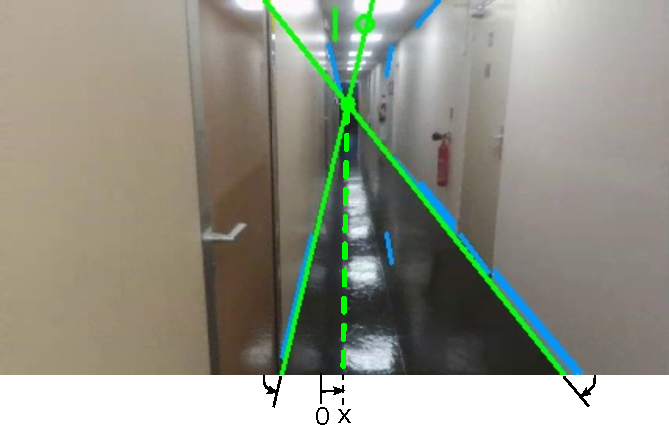
\includegraphics[width=\textwidth]{visudrone.pdf}
	\end{minipage}
	\begin{minipage}{0.5\textwidth}
	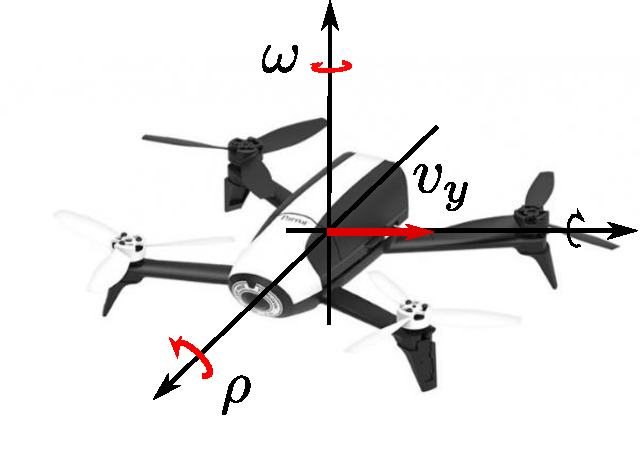
\includegraphics[width=\textwidth]{dronesteup}
	\end{minipage}
	\caption{Disposition des capteurs utilisés pour l'expérience}
	\label{fig:drone}
	\end{figure}

\begin{figure}
	\centering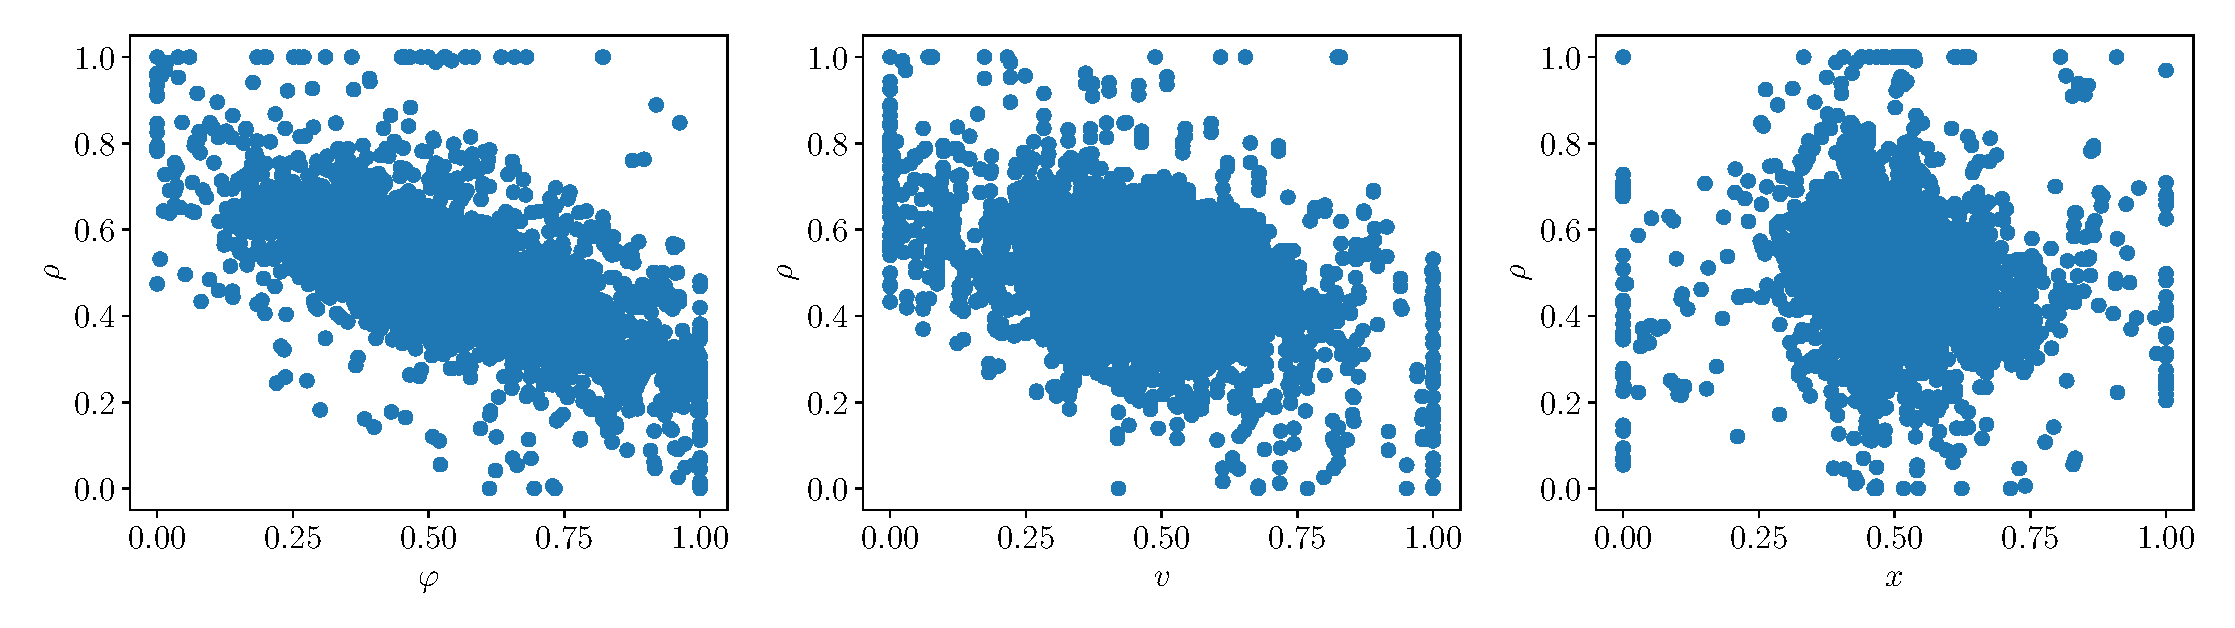
\includegraphics[width=\textwidth]{drone_inputs}
	\caption{Disposition et dépendances des entrées d'apprentissage. Nous chercherons à prédire $\rho$~: cette valeur dépend bien des autres modalités $v$, $\varphi$ et $x$. La dépendance est très simple (linéaire) mais très bruitée. \label{fig:drone_inp}}
\end{figure}


\subsection{Résultats}

La carte associée à $\rho$ possède une couche de poids externe et trois couches de poids contextuels. 
Ces poids sont représentés en figure \ref{fig:drone_w}. 

Nous observons d'abord que l'organisation des poids contextuels rappelle celle observé dans des conditions géométriques~: les poids contextuels définissent des zones. 
Ces zones sont moins précisément définies que la configuration sur un cercle, certainement à cause de la grande variabilité des données~: le modèle d'entrée est très bruité.

A chaque pas de temps, les valeurs $v$, $x$ et $\varphi$ sont récupérées~; le BMU est cherché par une phase de relaxation, puis la prédiction de la commande $\rho$, le poids externe du BMU dans la carte correspondante, est envoyé comme commande au drone.
La figure~\ref{fig:drone_w} présente ainsi en violet la valeur de l'activité contextuelle de la carte $\rho$, utilisée comme activité globale, lorsque la relaxation est terminée. Le BMU est pris au maximum de l'activité, $\bmu = 0.41$. Cela correspond à une valeur de commande $\w_e(\bmu\m{\rho}) = 0.49$. Cette valeur est remise à l'échelle et envoyée au drone.

L'expérience en temps réel montre que l'architecture de cartes réagit correctement aux entrées et envoie une commande cohérente au drone. Le drone apparaît voler correctement dans le couloir sans toucher les murs. Nous observons cependant une imprécision sur la trajectoire. La prédiction est donc correctement réalisée, toutefois assez imprécise. Cependant, le fait que les entrées soient très bruitées peut aussi expliquer le manque de précision. 
En figure \ref{fig:pred_drone}, nous avons représenté l'erreur de prédiction de l'architecture en effectuant une phase de test sur les mêmes données d'entrainement afin d'illustrer la qualité de la prédiction. Cette figure confirme que la prédiction est correctement effectuée mais très bruitée.

Cette capacité de prédiction montre une possibilité d'application des architectures de cartes sur des données réelles. Nous avons utilisé ici une architecture de quatre cartes, contrairement aux parties précédentes ou nous avons seulement utilisé des architectures de deux et trois cartes. 
L'apprentissage a été effectué seulement sur 4890 points que nous avons présentés une seule fois.
Les résultats des expériences montrent donc que les comportements des architectures de deux et trois cartes sont encore observés sur 4 cartes, apprenant sur des données très bruitées.
Peu d'itérations sont nécessaires en pratique pour déplier des cartes 1D. Rappelons que les poids externes et contextuels sont appris en une seule et même étape.
Enfin, la réactivité de l'envoi de la commande au drone montre donc que le nombre de pas de relaxation est assez faible et donc que la relaxation permet une réponse en temps réel, sans chercher une réactivité instantanée.
Ces observations, bien que sur un cas simple d'entrées en une dimension laissent la porte ouverte à une application possible des architectures CxSOM en pratique, par exemple en robotique.

Du travail supplémentaire est cependant nécessaire pour une réelle application de l'architecture. Cette expérience se place comme une première illustration du modèle dans un cadre réel.
Tout d'abord, il serait intéressant d'étudier l'application sur des données moins bruitées et disponibles en simulation afin de mesurer l'erreur de prédiction relative à l'architecture, comme une étape intermédiaire entre les données géométriques et le cadre réel. 
Plus généralement, les entrées d'une application robotique sont en pratique en plus grande dimension, par exemple une représentation d'une image.
Il sera nécessaire d'étudier l'organisation des cartes sur ce type de données, en utilisant dans ce cadre des cartes en deux dimensions.

\begin{figure}
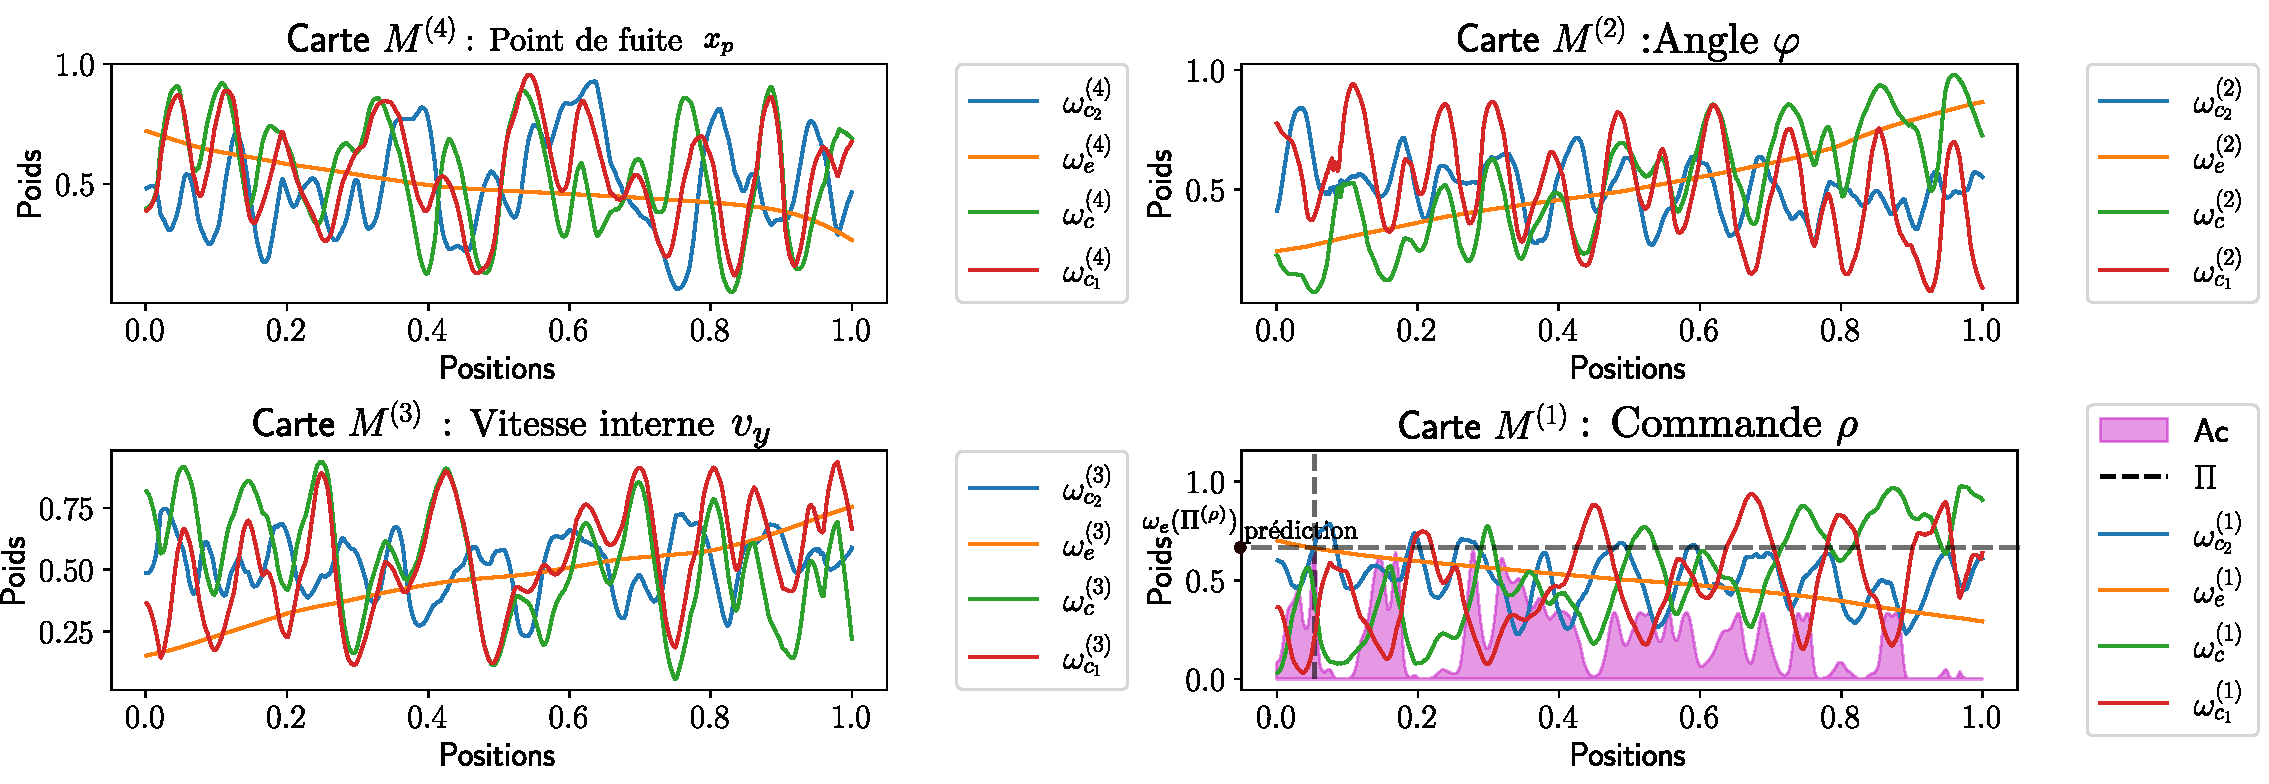
\includegraphics[width=\textwidth]{drone_weights.pdf}
\caption{Disposition des poids des 4 cartes après apprentissage.}
\label{fig:drone_w}
\end{figure}

\section{Conclusion}

Dans ce chapitre, nous avons d'abord observé que l'apprentissage du modèle d'entrée dans une architecture CxSOM passe par la formation de zones de poids contextuels créant une seconde échelle d'indices et donc de quantification vectorielle au sein de chaque carte. Ces zones ont été observées dans chaque carte sur toutes les dispositions d'entrées en deux et trois dimensions étudiées, dès lors que deux points différents du modèle d'entrées correspondent à la même entrée externe d'une carte.
Ces zones de poids contextuels encodent l'information sur le modèle $U$ dans chaque carte. Elles permettent à une carte de l'architecture d'acquérir un comportement prédictif en l'absence de son entrée externe. Une carte ne recevant pas d'entrée externe possède quand même un BMU grâce à ses activités contextuelles. Nous avons montré que le poids externe de ce BMU correspond bien à la valeur de l'entrée externe manquante. Cette prédiction est directement due à la présence des zones poids contextuelles.
Cette capacité de prédiction, avant d'être une application possible des cartes, permet d'évaluer l'apprentissage du modèle d'entrée par l'architecture.

Cette étude se veut l'identification de comportements élémentaires de cartes, dans le but de construire des architectures comportant plus de cartes. Dans de telles architectures, la disposition des connexions est un degré de liberté supplémentaire pour la conception de l'architecture.
Nous avons identifié sur l'exemple des cartes connectées en boucle que des connexions distantes dans l'architecture jouent bien un rôle dans l'activité d'une carte, tout en perdant leur influence. Par ailleurs, les observations réalisées sur le drone et sur l'architecture de 10 cartes montrent qu'une entrée ne participant pas à la définition du modèle ne vient pas polluer l'apprentissage. Au contraire, il semble même que les connexions de l'architecture reliée à la carte prenant cette entrée inutile apprennent à effacer leur participation au calcul de l'activité des autres cartes.
Une étude plus générale de l'influence des connexions permettra d'ajouter cette dimension à la conception de systèmes CxSOM.

Une perspective d'étude nécessaire est d'évaluer la distribution de l'encodage du modèle d'entrée dans les cartes. 
Dans les expériences présentées dans ce chapitre, plus globalement dans cette thèse, le modèle $U$ est une variable 1D. 
Nous avons montré que l'apprentissage se traduit par le fait que $U$ est une fonction de $\bmu$ dans chaque carte.
Dans une grande architecture, donc des entrées multimodales de dimension totale supérieure, on ne peut pas attendre que chaque carte encode complètement $U$~: le nombre de n\oe{}uds est limité et l'architecture se contenterait d'apprendre la valeur moyenne de $U$, comme dans l'architecture de 10 cartes pour $U$ de dimension 10.
On voudrait donc que $U$ ait une représentation distribuée au travers des cartes de l'architecture. 
Cette distribution de la représentation de $U$ n'apparaît pas clairement dans les expériences sur deux et trois cartes.
Cet aspect distribué de l'apprentissage est un point à étudier et si besoin à corriger en adaptant les paramètres du modèle pour envisager un développement du modèle CxSOM à grande échelle. Il sera par exemple possible de jouer sur les connexions, les paramètres des cartes ou le calcul d'activité.
Par exemple, nous avons toujours pris la  même valeur de $r_c$ pour toutes les couches de poids contextuels dans toutes les cartes. Ces paramètres et leur disposition constituent de nombreux degrés de libertés supplémentaires dans la construction d'une architecture et sont des pistes possibles d'étude et d'adaptation de l'architecture.


Enfin, toutes ces expériences ont été menées sur des cartes 1D apprenant à représenter des données en une dimension. Ce cas de figure est rarement rencontré en pratique et il serait intéressant d'évaluer l'apprentissage sur des dimensions d'entrées supérieures. Pour une tâche de quantification vectorielle classique par une SOM, il est plus pertinent d'utiliser des cartes en deux dimensions. Nous chercherons donc également à utiliser des cartes 2D dans une architecture CxSOM. Le passage de 1D à 2D n'est pas immédiat et pose de nombreuses questions quant à l'organisation des poids et la recherche de BMU par relaxation. 
Nous présenterons à ce propos à la fin de ce manuscrit des expériences préliminaires étudiant l'organisation des poids dans une architecture de cartes en deux dimensions.

\ifSubfilesClassLoaded{
    \printbibliography
    %\externaldocument{../main.tex}   
}{}
\end{document}